\documentclass[twoside]{book}

%% Encoding and language
	\usepackage[utf8]{inputenc}
	\usepackage[english,italian]{babel}

%% Graphics
	\usepackage[usenames,dvipsnames]{color}
	\usepackage{graphics}
	\usepackage{graphicx}
	\usepackage{subfig}
	\usepackage{wrapfig}
	\usepackage{sidecap}
	\usepackage{eso-pic}
	\usepackage{tikz}
	\usetikzlibrary{shapes,decorations}

	\graphicspath{{img/}}

%% Symbols and math
	\usepackage{textcomp}
	\usepackage{amsmath}
	\usepackage{amssymb} %needed for boxes with tikz
	\usepackage{upgreek}
	\usepackage[amssymb]{SIunits}
	\usepackage{xfrac}
	\usepackage[all]{xy} %needed for block diagrams

%% %%%%%%%
%% Layout
	\usepackage{multicol}
	\usepackage{framed}
	\usepackage{fancybox}
	\usepackage{fancyvrb}
	\usepackage[left=3cm,right=2cm,vmargin=2cm]{geometry}

	\usepackage{multirow} %% multirow tables
	\usepackage{booktabs} %% quality tables
	\newcommand {\otoprule}{\midrule[\heavyrulewidth]} % defines a customized height for the row under tables heading

	\usepackage{array}
	\usepackage{ulem}
	\usepackage{fancyhdr}
	\usepackage{dirtree}
	\usepackage{epigraph}

	\usepackage[unicode=true,bookmarks=true,bookmarksnumbered=false,bookmarksopen=false,breaklinks=true,pdfborder={0 0 0},backref=false,colorlinks=true]{hyperref}
	\hypersetup{pdftitle={GRASS GIS per gli archeologi},pdfauthor={Francesco de Virgilio}}

	\usepackage{listings}
	\lstset{ %
	basicstyle=\footnotesize,       % the size of the fonts that are used for the code
	numbers=left,                   % where to put the line-numbers
	numberstyle=\footnotesize,      % the size of the fonts that are used for the line-numbers
	stepnumber=1,                   % the step between two line-numbers. If it's 1 each line will be numbered
	numbersep=5pt,                  % how far the line-numbers are from the code
	backgroundcolor=\color{white},  % choose the background color. You must add \usepackage{color}
	showspaces=false,               % show spaces adding particular underscores
	showstringspaces=false,         % underline spaces within strings
	showtabs=false,                 % show tabs within strings adding particular underscores
	frame=single,	                % adds a frame around the code
	tabsize=2,	                % sets default tabsize to 2 spaces
	captionpos=b,                   % sets the caption-position to bottom
	breaklines=true,                % sets automatic line breaking
	breakatwhitespace=false,        % sets if automatic breaks should only happen at whitespace
	%title=,                         % show the filename of files included with \lstinputlisting; also try caption instead of title
	escapeinside={\%*}{*)},         % if you want to add a comment within your code
	morekeywords={*,\dots}          % if you want to add more keywords to the set
	}

	\usepackage{setspace}
	\onehalfspacing

	%% header con fancyhdr
	\pagestyle{fancy}
	\lhead{}
	\chead{}
	\rhead{\bfseries \leftmark}
	\cfoot{GRASS GIS in archeologia}
	\rfoot{\thepage}
	\renewcommand{\headrulewidth}{0.4pt}
	\renewcommand{\footrulewidth}{0.4pt}
	\renewcommand{\chaptermark}[1]{\markboth{#1}{}}

	\normalem %definisce lo stile delle sottolineature
	\VerbatimFootnotes %abilita l'utilizzo del codice nelle note, con il pacchetto fancyvrb

%% </Layout>
%% %%%%%%%%%%

\begin{document}
	\frontmatter
	\newcommand\BackgroundPicA{
	\put(140,220){{
		\begin{tikzpicture}
		\node[opacity=0.5]{\includegraphics[scale=5.5]{logo-book}};
		\end{tikzpicture}
}}}

\newcommand*{\titleTH}{\begingroup
	\raggedleft
	\definecolor{shadecolor}{gray}{0.75}
	\vspace*{\baselineskip}
	\hrule \vspace*{0.5cm}
	{\bfseries \Large \fontsize{8mm}{10mm}\selectfont Introduzione all'utilizzo di}\\[\baselineskip]
	{\textcolor{red}{\Huge \fontsize{15mm}{17mm}\selectfont GRASS GIS}}\makebox[0in][l] {\scalebox{1}[-1]{\textcolor{shadecolor}{{\large \fontsize{8mm}{10mm}\selectfont{\textsl{ in Archeologia}}}}}}{\textcolor{red}{\large \fontsize{8mm}{10mm}\selectfont{\textsl{ in Archeologia}}}}\par
	\vspace{10pt}
	\AddToShipoutPicture*{\BackgroundPicA}
	\vfill
	\includegraphics[width=0.1\textwidth]{img/oia-logo}\par
	\vspace{10pt}
	{\Large O.I.A.}\par
	{\normalsize Open Idea for Archaeology}\\
	{\footnotesize Francesco de Virgilio and the\\grass-arch project contributors}\par
	\vspace*{3\baselineskip}
\endgroup}
\thispagestyle{empty}
\titleTH

\pagebreak{}

\pagenumbering{roman}~

\pagebreak{}

\vspace*{4cm}


\epigraph{«Sed omnia praeclara tam difficilia, quam rara sunt.»\\ \medskip{}Tutte le cose eccellenti sono tanto difficili, quanto rare.}{\emph{Etica, De potentia intellectus seu de libertate humana, Propositio XLII, scholium}\\ \textsc{Baruch Spinoza}}

	\pagebreak
	\tableofcontents
	\pagebreak
	\listoffigures
	\pagebreak
	\chapter*{Prefazione}

	Questo manualetto nasce dall'esigenza, interna alla Cattedra di Archeologia Medievale dell'Università degli Studi di Bari, di affrontare il problema della documentazione archeologica degli scavi del sito medievale di Siponto (FG).\\

	La progressiva informatizzazione di tutta la documentazione archeologica collezionata in anni di attività ha portato alla necessità di affrontare la gestione del dato elettronico in maniera quanto più possibile flessibile ed economica allo stesso tempo. In questo contesto, GRASS GIS rivela la sua estrema utilità. Una delle caratteristiche del software che gli archeologi apprezzeranno maggiormente è sicuramente la possibilità di gestire una quantità enorme di dati, con un'avidità di potenza di calcolo decisamente ridotta, al contrario di altri software con caratteristiche affini, rilasciati in licenza libera e non (ArchView, Quantum GIS, ecc.).

	La flessibilità di GRASS GIS permette di gestire un numero impressionante di differenti formati di dati, e di creare complesse elaborazioni, pur tuttavia passando per una gestione del dato non eccessivamente complessa. A differenza di altri sistemi GIS, GRASS ha una curva d'apprendimento molto più ripida rispetto ad altri software, situazione che tuttavia è indice di una eccezionale potenza intrinseca, derivante dai circa 400 moduli eseguibili che lo compongono, e dei risultati professionali che si possono ottenere.

	Questo manualetto è orientato ad un pubblico che ha già acquisito una certa familiarità con almeno un sistema GIS, e cerca di affrontare le problematiche più importanti nella gestione del dato archeologico.  L'approccio di GRASS GIS alla risoluzione di alcuni problemi può alle volte sembrare inutilmente macchinoso, ma si scoprirà essere sorprendentemente pratico e veloce una volta acquisita familiarità con la maniera di operare caratteristica del software; soprattutto, GRASS si rivela estremamente utile quando si ha necessità di operare in maniera precisa e consapevole su grandi quantità di dati, come può avvenire durante (o dopo) uno scavo archeologico.

	In questa sede, soprattutto per la grande quantità di documentazione disponibile sui sistemi GIS e su GRASS in particolare, si eviteranno ripetizioni di materiale già pubblicato da altri autori, limitando molti argomenti ad un semplice richiamo. Al termine del manuale, nella Bibliografia, sono disponibili tutti i riferimenti per approfondire le caratteristiche dei sistemi GIS, dell'analisi geografica e territoriale, e sull'utilizzo di GRASS.

	Inoltre, particolare da non trascurare soprattutto in ambito didattico, GRASS GIS è rilasciato in licenza libera (GNU GPL): ciò consente non solo di poter ottenere il software gratuitamente (scaricandolo liberamente dalla rete internet) ma anche di utilizzarlo e di aggiornarlo senza alcun costo di licenza, così come di distribuirlo senza alcun onere a tutti gli studenti. Inoltre, la completa documentazione disponibile online, a cura dello stesso team di sviluppo del software, permette a tutti di avere accesso alle spiegazioni dettagliate sull'utilizzo dei moduli che compongono il programma (senza la necessità di acquisto di manuali aggiuntivi). In ultima analisi, gli utenti più esperti hanno la possibilità di ``estendere'' il software con lo sviluppo di moduli e script personalizzati, per agevolare alcune operazioni ripetitive o per adattare il software di analisi geospaziale alle proprie peculiari esigenze (sono note applicazioni che vanno dall'ingegneria delle reti idriche a quella delle reti stradali, passando per le analisi meteorologiche). Inoltre, GRASS può essere incorporato all'interno di altri programmi che possono fungere da interfaccia utente come ad esempio, Quantum GIS, rispetto al quale ha anche il vantaggio di gestire in un unico layer sia punti che linee che poligoni, facilitando il lavoro di gestione del dato archeologico.\\

	L'utilizzo di GRASS GIS in ambito archeologico segna un ulteriore passo avanti sulla strada della ricerca di standard all'interno della documentazione archeologica, ricerca che si è affermata di pari passo con l'introduzione dell'\emph{archeoinformatica}, disciplina tesa all'applicazione delle metodologie e delle strumentazioni informatiche all'archeologia stratigrafica e all'archeologia quantitativa (in quest'ultimo contesto, GRASS offre potenti strumenti di analisi statistica). Quindi, se a livello di documentazione di scavo non esiste attualmente veramente nessuno standard informatico, certamente per tutto quello che riguarda l'archeologia dei paesaggi e il telerilevamento GRASS è al passo con qualunque altro software proprietario nella gestione e nell'analisi di immagini aeree, dati LIDAR, \emph{et similia}.

	L'adozione di standard, in tutti i campi della ricerca scientifica, è un concreto aiuto alla comunicazione e divulgazione dei risultati.  Tuttavia, la ricerca di standard internazionali dovrebbe passare sia per l'utilizzo di standard aperti, sia attraverso l'impiego di software open source: in entrambe queste affermazioni risiede la coscienza di fondo che la ricerca storica -- ed in particolare quella archeologica -- non può essere appannaggio di pochi, ma deve innescare un processo che vada dallo studio delle fonti, alla ricerca sul campo, all'analisi dei risultati; il processo deve concludersi con una divulgazione che consenta all'Uomo di conoscere e comprendere la propria Storia e quella del luogo in cui vive, per sviluppare una nuova cultura della comprensione e trasmissione al futuro del patrimonio storico.\\

	L'utilizzo di GRASS in archeologia\footnote{Si faccia ad esempio riferimento al \href{http://grass.osgeo.org/wiki/Archeology}{wiki ufficiale di GRASS}.}, al 2009, può vantare innumerevoli campi d'applicazione, spesso mai raggiunti da software proprietari: si guardi ad esempio il lavoro presentato al GRASS Meeting del 2006 da parte di Arc-Team s.n.c.\footnote{Reperibile da \href{file:http://www.dimset.unige.it/eventi/grass/presentazioni/sessione 3/bezzi et al.pdf}{http://www.dimset.unige.it/eventi/grass/presentazioni/sessione 3/bezzi et al.pdf}.} sull'utilizzo dei \emph{voxel} (raster 3D) per la gestione di dati archeologici di scavo, poi ripresi sempre da Arc-Team e da Undine Lieberwirth (quest'ultima al workshop "Archaeologie~und~Computer" di Vienna del 2006\footnote{\emph{Workshop 11 Archaeologie und Computer, Kulturelles Erbe und Neue Technologien} - Wien, Aramus 2006, la prima spedizione archeologica internazionale ad utilizzare soltanto Software Libero.}). I lavori di Emanuel Demetrescu sull'archeologia urbana di Roma\footnote{Le diapositive dell'intervento sono disponibili presso il \href{file:http://www.perseo.lettere.unipd.it/workshop08/lib/exe/fetch.php?id=download&cache=cache&media=workshop08:documenti:demetrescu_lic.odp}{portale} dell'Università degli Studi di Padova.} sono certamente uno degli esempi più sorprendenti delle grandi potenzialità di GRASS (e dei software connessi) applicati ad un caso di archeologia reale, tra l'altro con risultati interessanti anche al di là delle sperimentazioni tecniche. Infine, del team di sviluppo di GRASS fa parte Michael Barton, archeologo/antropologo statunitense che svolge ricerche territoriali sia oltreoceano sia in Spagna. A livello italiano, risulta inoltre molto preziosa la testimonianza offerta nel secondo volume della collana ``Metodi e temi dell'archeologia medievale'', ampiamente descritta nel volume ``Informatica ed Archeologia Medievale -- L'esperienza senese'' (esperienza che ha previsto anche l'utilizzo dei software open source GRASS e QuantumGIS)\footnote{\emph{Metodi e temi dell'archeologia medievale}, vol. 2, ``Informatica e Archeologia Medievale --- L'esperienza senese'', a cura di Vittorio Fronza, Alessandra Nardini, Marco Valenti.}.\\

	Un ringraziamento va a tutte le persone che hanno mostrato interesse e dedicato tempo ed energie alla sperimentazione di software libero in ambito archeologico, in particolare al Dott.~Austacio~Busto ed alla Dott.ssa~Raffaella~Palombella; un enorme ringraziamento è rivolto a Paola~Monno, prima lettrice del manuale, per i suoi preziosi consigli; si ringraziano inoltre per la preziosa collaborazione: Stefano Costa, Luca Delucchi, Luca Mandolesi, Francesco Lovergine. Ovviamente qualsiasi consiglio, considerazione o critica sono benaccetti, all'indirizzo \href{mailto:fradeve11@gmail.com}{fradeve11@gmail.com}.
	\vfill
	La prima versione di questo documento è stata realizzata nel contesto del progetto ``Siponto Aperta'', lanciato dall'associazione culturale O.I.A. -- Open Idea for Archaeology, progetto n. 528 vincitore dell'edizione 2010 del concorso ``Bollenti Spiriti -- Principi Attivi''.\\~\\
	\includegraphics[width=0.4\textwidth]{img/logo-pa/c_Logo_vincitore_orizz}\hfill
	\includegraphics[width=0.2\textwidth]{img/logo-pa/b_Logo_Regione}


	\mainmatter
	%\pagenumbering{arabic}
%\setcounter{page}{1}

\chapter{Introduzione al GIS}

\begin{wrapfigure}{O}{0.5\columnwidth}
	\begin{centering}
		\includegraphics[scale=0.35]{img/500px-Simple_vector_map}
		\par
	\end{centering}
	\caption{{\small\label{fig:Una-semplice-mappa}Una semplice mappa vettoriale, che usa tutti i tre elementi delle geometrie: i punti vengono usati per rappresentare i pozzi, le linee per schematizzare i fiumi e un poligono descrive il lago.}}
	\vspace{-10pt}
\end{wrapfigure}

Per definizione, un \emph{Sistema Informativo Geografico} (SIT) o \emph{Geographic Information System} (GIS) in inglese, è un \emph{sistema informatico per l'acquisizione, conservazione, analisi e visualizzazione di dati geografici}. Viene definito sistema in quanto costituito da un insieme di componenti (hardware, software ed umane) che interagiscono tra loro, per dare vita alla caratteristica principale di un GIS: gestire dati geografici o georeferenziati, ovvero dati relativi ad elementi od oggetti della superficie terrestre la cui posizione è definita da un insieme (non necessariamente una coppia) di coordinate. Rispetto ad una rappresentazione puramente geometrica degli oggetti, il GIS deve memorizzare i dati descrittivi (\emph{attributi}) dei singoli oggetti reali, in tabelle: ogni riga si riferisce ad un singolo oggetto e ogni colonna ad un singolo attributo. Ogni GIS è dunque basato su un modello del mondo reale definito per la specifica applicazione; tale concetto verrà meglio definito successivamente.

\section{Il modello dei dati
%\footnote{Geographic information system. (2009, August 26). In Wikipedia, The Free Encyclopedia. Retrieved 15:10, August 26, 2009, from http://en.wikipedia.org/w/index.php?title=Geographic\_information\_system\&oldid=310176131}
}

	Un sistema GIS è una formalizzazione degli oggetti presenti nella realtà; per descrivere correttamente gli oggetti reali distribuiti sulla superficie terrestre, è indispensabile che siano caratterizzati da:
	
	\begin{description}
		\item [{geometria}] riproduce la forma degli oggetti e viene ricondotta a tre elementi (schematizzati in fig. \ref{fig:Una-semplice-mappa}), definiti da \emph{vettori}:

			\begin{description}
				\item [{punti}] sono entità adimensionali usate per elementi geografici che possono essere espressi da un singolo punto (può essere il caso della sommità di una collina o di una montagna, o della posizione di un albero); il concetto di informazione puntuale è strettamente legato al rapporto tra estensione dell'elemento ed estensione dell'area in analisi\footnote{Ad esempio, se si sta analizzando la posizione degli alberi monumentali su un'estensione di 4 ettari, ogni albero sarà simboleggiato da un punto; invece, se si sta analizzando l'area coperta da alberi monumentali in un giardino di \unit{\meter\squared} di area, ogni albero sarà rappresentato non più da un punto, ma da un'area.};
				\item [{linee}] o polilinee, sono entità monodimensionali utilizzate per descrivere strutture lineari (ad esempio fiumi, strade, ferrovie, ecc.); è altresì valido per le linee il concetto di rapporto tra estensione dell'elemento e dell'area;
				\item [{poligoni}] o aree, sono usati per descrivere entità che ricoprono una certa area dell'estensione terrestre, come laghi, confini di parchi naturali, città, palazzi, ecc.; dall'informazione poligonale è possibile ricavare sia la misura di un perimetro che quella dell'area coperta dal poligono stesso. 
			\end{description}
			
			Due considerazioni importanti a proposito della geometria:
		
			\begin{itemize}
				\item Ognuna di queste geometrie è definita, all'interno del database geografico, da una riga, ovvero da un \emph{record} di dati, che descrive i suoi attributi.
				\item Le diverse geometrie possono essere comparate tra loro, o messe in rapporto ad altri elementi di differenti geometrie; ade esempio, è possibile ottenere facilmente un confronto tra l'area di ciascun lago, così come un elenco di tutti i picchi montuosi a meno di 10 km dal centro del lago.
			\end{itemize}

		\item [{topologia}] è l'insieme delle informazioni che riguardano le relazioni spaziali reciproche tra i diversi elementi della geometria, come la \emph{connessione}, l'\emph{adiacenza} o l'\emph{inclusione}. Permette ad esempio di specificare se una linea è connessa ad un'altra o se semplicemente si sovrappongono senza comunicare (schematizzazione di due strade che possono intersecarsi a formare un incrocio o sovrapporsi in un cavalcavia). I dati vettoriali generati dalle geometrie possono essere gestiti in maniera tale che siano rispettate le \emph{regole topologiche}, come ad esempio ``i poligoni non devono sovrapporsi''. I dati vettoriali individuati dalle geometrie e nel rispetto delle regole topologiche, possono rappresentare astrazioni più o meno complesse della superficie terrestre, come ad esempio l'elevazione del terreno, rappresentata tramite un insieme di poligoni (triangoli) adiacenti i cui vertici sono disposti nelle tre dimensioni dello spazio.
		
		\item [{attributi}] sono dati che descrivono gli oggetti reali, associati alle rappresentazioni geometriche di quegli oggetti nel GIS. Per esempio, una database che descrive dei laghi può contenere informazioni aggiuntive collegate alle semplici informazioni geografiche sulla geometria dei laghi, come la loro profondità massima, il grado di salinità, la presenza di sostanze inquinanti,ecc.. Queste informazioni possono essere utilizzate per generare una mappa tematica con l'obiettivo di descrivere un particolare attributo del set di dati, tra quelli citati sopra; ad esempio, i laghi possono essere colorati in funzione del livello di inquinamento.

	\end{description}

\section{La rappresentazione dei dati}
	Nel GIS esistono due tipi di rappresentazione dei dati, ``vettoriale'' (\emph{vector} in inglese) e ``raster'' (un esempio in fig. \ref{fig:A-sinistra,-rappresentazione}). Nella rappresentazione \textbf{vettoriale}, introdotta precedentemente, ogni punto è definito da una coppia di coordinate (se questo punto è parte di una linea o di un poligono, si avrà un insieme di coppie di coordinate, che individuano i vari punti, connessi tra loro con segmenti retti che formano la rappresentazione grafica dell'elemento). Generalmente i punti alle estremità di una linea vengono definiti \emph{nodi}, mentre quelli intermedi \emph{vertici}.\\ Nella rappresentazione \textbf{raster}, l'area considerata è suddivisa in un insieme di celle, solitamente di forma quadrata, in ciascuna delle quali viene registrato l'attributo (o categoria) presente, sotto forma di valore numerico, come si vede in fig.~\ref{fig:Listato-di-un-raster}.\\
	
	\begin{figure}
		\centering
			\begin{minipage}[c][1\totalheight][t]{0.5\columnwidth}

				\begin{center} \texttt{north: 15} \end{center}
				\begin{center} \texttt{south: 0} \end{center}
				\begin{center} \texttt{east: 15} \end{center}
				\begin{center} \texttt{west: 0} \end{center}
				\begin{center} \texttt{rows: 15} \end{center}
				\begin{center} \texttt{cols: 15} \end{center}

				\begin{spacing}{0.3}
					\begin{center} \texttt{3 3 1 1 1 1 1 1 1 3 3 3 3 3 3} \par\end{center}
					\begin{center} \texttt{3 3 1 1 1 1 1 1 1 3 3 3 3 3 3} \par\end{center}
					\begin{center} \texttt{3 3 1 1 1 1 1 1 1 3 3 3 3 3 3} \par\end{center}
					\begin{center} \texttt{3 3 1 1 1 1 1 1 1 3 3 3 3 3 3} \par\end{center}
					\begin{center} \texttt{2 2 2 2 2 2 2 2 2 2 2 2 2 2 2} \par\end{center}
					\begin{center} \texttt{2 2 2 2 2 2 2 2 2 2 2 2 2 2 2} \par\end{center}
					\begin{center} \texttt{2 2 2 2 2 2 2 2 2 2 2 2 2 2 2} \par\end{center}
					\begin{center} \texttt{3 3 1 1 1 1 1 1 1 1 1 1 1 3 3} \par\end{center}
					\begin{center} \texttt{3 3 1 1 1 1 1 1 1 1 1 1 1 3 3} \par\end{center}
					\begin{center} \texttt{3 3 1 1 1 1 1 1 1 1 1 1 1 3 3} \par\end{center}
					\begin{center} \texttt{3 3 1 1 1 1 1 1 1 1 1 1 1 3 3} \par\end{center}
					\begin{center} \texttt{3 3 1 1 1 1 1 1 1 1 1 1 1 3 3} \par\end{center}
					\begin{center} \texttt{3 3 3 3 3 3 3 3 3 3 3 3 3 3 3} \par\end{center}
					\begin{center} \texttt{3 3 3 3 3 3 3 3 3 3 3 3 3 3 3} \par\end{center}
					\begin{center} \texttt{3 3 3 3 3 3 3 3 3 3 3 3 3 3 3} \par\end{center}
				\end{spacing}
			\end{minipage}
		\caption{{\small\label{fig:Listato-di-un-raster}Listato di un raster esportato in formato testuale. Idealmente, in questo listato ogni ``cella'' della griglia è rappresentata da un numero, il cui valore definisce la caratteristica della cella.}}
	\end{figure}

	\begin{figure}
		\centering
		\includegraphics[scale=0.1]{img/Raster_vector_gis}
		\caption{{\small\label{fig:A-sinistra,-rappresentazione}A sinistra, rappresentazione di dati vettoriali, a destra gli stessi dati informato raster.}}
	\end{figure}
	
	Essenzialmente è un raster ogni tipo di immagine digitale costituita da una griglia di informazioni, divisa quindi in celle che definiscono una struttura di righe e colonne. Chiunque abbia familiarità con la fotografia digitale riconosce nel \emph{pixel} la minima unità dell'immagine digitale e quindi l'elemento essenziale della griglia; un insieme di pixel da origine ad un'immagine, differente per questo da un dato di tipo vettoriale. Anche un'immagine raster rappresenta un'astrazione della realtà, perché ogni pixel è colorato in funzione della zona che rappresenta. La risoluzione di un'immagine raster è data dalla dimensione della sua cella in unità del suolo. Le immagini aeree, le ortofoto o le immagini satellitari sono tipi di raster comunemente utilizzati in software GIS, con l'obiettivo di fornire un'immagine dettagliata del territorio, che poi verrà digitalizzata ``disegnando'' su di essa una rappresentazione schematica vettoriale.  Altre tipologie di raster possono contenere informazioni selettive: per esempio, ogni pixel può essere colorato in funzione della sua altitudine (in questo caso si ha un modello di elevazione digitale o \emph{DEM}); altri raster possono contenere informazioni sulla riflessione della luce secondo particolari lunghezze d'onda (dati \emph{LANDSAT}), o secondo la temperatura. Le celle --- pixel --- che costituiscono le immagini possono contenere quindi vari tipi di informazioni sotto forma di diversi colori. È possibile realizzare tali tipologie di raster grazie a delle convenzioni che definiscono una certa scala di colori per rappresentare ben determinate tipologie di informazioni, ad esempio la nota RGB (\emph{red}, \emph{green}, \emph{blue} --- rosso, verde, blu). All'interno di file raster è anche possibile che siano presenti pixel vuoti, rappresentanti porzioni di territorio per le quali il dato in analisi non è disponibile; tali pixel prendono spesso il nome di \emph{null}. I dati raster vengono memorizzati in diversi formati, a partire da una struttura standard sotto forma di file (nel caso di TIF, JPEG, ecc.) fino a grandi quantità di dati raster binari (BLOB) immagazzinati in un sistema di gestione di un database relazionale (RDBMS), in un'impostazione simile a quella di dati vettoriali\footnote{Un insieme di dati archiviati in un database, se opportunamente gestiti, permettono generalmente una gestione più veloce dei dati raster, ma richiedono la registrazione di milioni di \emph{record} all'interno del database (approssimativamente uno per ogni pixel).}.

	\chapter{Elementi di GRASS GIS}

\section{Informazioni generali%
%\footnote{GRASS GIS. (10 giugno 2009). Wikipedia, L'enciclopedia libera. Tratto il 26 agosto 2009, 15:41 da http://it.wikipedia.org/w/index.php?title=GRASS\_GIS\&oldid=24604028.}
}

	\begin{wrapfigure}{o}{0.35\columnwidth}
		\centering
		\includegraphics[scale=0.15]{img/Grasslogo_vector_big}\par
		\caption{{\small Il logo di GRASS GIS.}}
	\end{wrapfigure}

	\textbf{GRASS} è l'acronimo di \textbf{G}eographic \textbf{R}esources \textbf{A}nalysis \textbf{S}upport \textbf{S}ystem. GRASS è un software libero di \emph{Geographical Information System} (GIS), rilasciato sotto la licenza GNU GPL. Esistono versioni per diverse piattaforme. GRASS nasce all'inizio degli anni '80 come progetto dell\textquoteright{}esercito degli Stati Uniti (\emph{US Army Corp of Engineering Research Laboratory} --- USACerl). Lo sviluppo avviene in particolare utilizzando il linguaggio C ed Unix come sistema operativo di riferimento. Nel 1996 l'esercito degli Stati Uniti prende la decisione di abbandonare lo sviluppo di GRASS. Gli utenti sono invitati a migrare verso sistemi commerciali, mentre l'ultima versione di GRASS (4.1) rimane nel pubblico dominio. Alla fine del 1997, dopo oltre un anno, riesce a formarsi un nuovo team internazionale che si fa carico di continuare lo sviluppo. L'aggiunta di nuovi moduli e porzioni di codice al software di pubblico dominio pone però il problema del diritto d'autore. Nell'ottobre 1999 dopo un'ampia discussione il GRASS Development Team (GDT) decide di rilasciare GRASS (5.0b) con la licenza GNU GPL. Attualmente il centro di sviluppo del software ha sede a Povo (Trento, Trentino --- Italia), presso l'ITC-irst, ma si avvale di molti collaboratori esterni. Il coordinatore del progetto è Markus Neteler.\\

	Tramite il sistema dei moduli, GRASS permette di utilizzare altri programmi quali

	\begin{description}
		\item [{PROJ.4}] libreria per le proiezioni cartografiche, usata in quasi i tutti i sistemi geografici liberi;
		\item [{OGR~Simple~Feature~Library}] gestione file vettoriali in diversi formati;
		\item [{GDAL}] (\emph{Geospatial Data Abstraction Library}), gestione file raster in diversi formati;
		\item [{R}] per gli aspetti statistici e di geostatistica.
	\end{description}
		
	GRASS GIS funziona sotto sistema operativo \emph{Unix} (o similari: GNU/Linux), sia su workstation che su personal computer e sotto sistema operativo \emph{Windows} mediante \emph{cygwin}, che simula l'ambiente Unix.


\section{Installazione su Ubuntu GNU/Linux\label{sec:Installazione-su-Ubuntu}}
	Questa guida è orientata all'utilizzo di GRASS su sistemi GNU/Linux, in particolare sulla distribuzione Ubuntu. Le seguenti indicazioni possono essere comunque applicate a qualsiasi distribuzione derivata da Debian GNU/Linux. Per ottenere GRASS è sufficiente installare i due pacchetti \texttt{grass} e \texttt{grass-doc}. È possibile farlo tramite terminale, con il comando \texttt{sudo apt-get install grass grass-doc} o tramite il gestore di pacchetti per GNOME, Synaptic. Per ulteriori informazioni su come installare software su Ubuntu si rimanda alla documentazione ufficiale della comunità italiana, presente online all'indirizzo \url{http://wiki.ubuntu-it.org/AmministrazioneSistema/InstallareProgrammi}. Si troverà anche molto utile l'installazione del software contenuto nel pacchetto \texttt{gdal-bin}.


\section{Caratteristiche principali\cite{uniparma}}

	\subsection{Gestione dei dati in GRASS}
		In GRASS ad ogni cella (pixel) che compone una carta raster, viene attribuito un solo valore di categoria ed eventualmente un'etichetta descrittiva. La non assegnazione di una categoria comporta l'assegnazione automatica di un valore particolare detto \emph{null}. La geometria di una carta vettoriale (uno dei due componenti oltre agli attributi) è riconducibile ad una delle cinque tipologie seguenti, che si discostano leggermente da quelle elencate precedentemente:
		
		\begin{description}
			\item [{point~(\emph{punto})}] per rappresentare gli elementi puntiformi (punti quotati, pozzi, ecc). Ogni punto è rappresentato da una coppia di coordinate.
			\item [{line~(\emph{linea})}] per rappresentare elementi lineari. Ogni linea è costituita da una \emph{spezzata}.
			\item [{boundary~(\emph{bordo})}] per rappresentare, anche parzialmente, i bordi di aree chiuse. È una spezzata memorizzata mediante una sequenza di coppie di coordinate in corrispondenza dei nodi e dei vertici.
			\item [{centroid~(\emph{centroide})}] è un elemento puntiforme all'interno di un'area chiusa in corrispondenza del quale vengono inseriti gli attributi dell'area; ogni centroide è rappresentato da una coppia di coordinate.
			\item [{area~(\emph{area})}] è l'insieme di un bordo di area (\emph{boundary}) completo (quindi chiuso) e del relativo centroide.
		\end{description}
		
		In GRASS, la geometria è salvata in un formato vettoriale specifico del programma (formato nativo), ma è comunque possibile importare e trasformare molti altri formati (ArcInfo-Coverages, CSV, SHAPE files, \emph{GIS ManagerL}, MapInfo, MySQL, ODBC, OGDI, PostgreSQL/PostGIS, S57, SDTS, TIGER, UK .NTF, VRT). Alcuni di questi formati (come lo shapefile) possono essere gestiti direttamente senza la conversione nel formato nativo. Come abbiamo considerato precedentemente, le informazioni vettoriali sono distinte nelle geometrie appena elencate e negli attributi. Geometrie ed attributi in GRASS vengono salvati separatamente in tabelle diverse, collegate tramite un valore univoco denominato \emph{cat}. Il collegamento tra geometrie ed attributi viene operato tramite una DBMI (\emph{DataBase Management Interface} -- Interfaccia di Gestione del DataBase). Attualmente GRASS gestisce i seguenti DBMI: DBF, PostgreSQL, MySQL, ODBC, mediante dei software interni (\emph{driver}), rispettivamente \emph{dbf}, \emph{pg} e \emph{ogr}. Il DBMI DBF è il driver di default: ciò significa che qualsiasi tipo di dato vettoriale importato in GRASS viene copiato dal software in una cartella di lavoro, e tutte le informazioni vengono trasferite in tabelle dbf in questa cartella. Vedremo in seguito com'è organizzata e come si gestisce la cartella di lavoro.\\

		La funzione della categoria (o colonna \emph{cat}) quindi è quella di fungere da {}``ponte'' tra le tabelle che contengono le coordinate geografiche dei vari punti che costituiscono le geometrie e gli attributi delle stesse geometrie, semplicemente conferendo agli attributi lo stesso valore di \emph{cat} delle geometrie che li presentano. La tabella \ref{tab:La-tabel} riassume questo concetto.

		\begin{table}
			\centering
			\input{tab/attributi}
			\qquad
			\input{tab/geometrie}
			\caption{\label{tab:La-tabel}{\small La tabella di sinistra sintetizza la struttura della tabella delle geometrie, contenente le coordinate dei punti e la loro topologia; la tabella a destra mostra come la colonna}\emph{\small cat}{\small{} determini il collegamento degli attributi (immagazzinati in un'apposita tabella) con le geometrie.}}
		\end{table}

		\input{tab/box_nomicarte}

	\subsection{Organizzazione dei dati}
		Una delle caratteristiche di GRASS rispetto ad altri software come Quantum GIS è l'estremo ordine con cui i dati vengono gestiti. Mentre la maggior parte dei software GIS si limita ad aprire i file mantenendoli nella loro posizione, quando un dato (di qualsiasi tipo) viene importato in GRASS, il programma ne crea una copia nella propria cartella di lavoro, elaborando i dati tramite il proprio driver predefinito (come precisato sopra, nella maggior parte dei casi il driver è il dbf). Con questa procedura automatica GRASS si crea automaticamente delle sottocartelle della propria cartella di lavoro, che può essere comunque posizionata a piacimento dell'utente su qualsiasi dispositivo (su una cartella in un PC locale o anche in un dispositivo di memorizzazione di massa come una penna USB). Comunque, in prima istanza, prima di poter operare, GRASS necessita che l'utente definisca una cartella ``radice'' in cui inserire tutti i dati. Nei sistemi operativi \emph{Unix} (come GNU/Linux) questa cartella viene posizionata in maniera predefinita nella \textsf{home} del sistema, per essere precisi nella cartella \textsf{grassdata} all'interno di \textsf{/home/nomeutente}. D'ora in poi assumeremo che la nostra cartella di lavoro sia appunto \textsf{/home/nomeutente/grassdata}.\\

		Esplorando il contenuto di una cartella di lavoro di GRASS, si noterà che essa è strutturata come nello schema \ref{tab:Organizzazione-schematica-della}.
		
		\begin{table}
			\begin{centering}
				\framebox{
					\begin{minipage}[t]{1\columnwidth}
						\dirtree{%
						.1 /home/nomeutente. 
						.2 grassdata. 
						.3 \underbar{location1}.\DTcomment{regione di lavoro}. 
						.4 PERMANENT.\DTcomment{mapset di base}. 
						.4 mapset1.\DTcomment{altri mapset$\downarrow$}. 
						.4 mapset2. 
						.4 mapset3. 
						.3 \underbar{location2}. 
						.4 PERMANENT. 
						.4 location1. 
						.4 location2. }
					\end{minipage}}
			\end{centering}
			\caption{{\small \label{tab:Organizzazione-schematica-della}Organizzazione schematica della cartella di lavoro di GRASS.}}
		\end{table}


		Le cartelle \textsf{location} sono create dall'utente, e rappresentano l'area su cui si intende operare. Per area è possibile considerare una qualsiasi estensione geografica (potenzialmente illimitata in estensione, sia in grande che in piccolo). Quindi, lavorando su uno scavo archeologico, una location potrebbe essere rappresentata dall'area di scavo, oppure --- parlando di uno scavo urbano d'emergenza --- dall'area dello scavo più l'area urbana nel raggio di 200 metri dal perimetro dello scavo. Anche le cartelle \textsf{mapset} vengono create dall'utente, e servono a immagazzinare le mappe. Non esiste alcun precetto che governi la gestione dei mapset, ma la loro struttura è tale da suggerire un utilizzo relativo ai tematismi: ogni tematismo va immagazzinato in un mapset. Dovendo gestire, ad esempio, un centinaio di tematismi, potrebbe comunque tornare utile unire più tematismi in un solo mapset.\\
		
		Un esempio pratico di come potrebbe essere organizzata una cartella di lavoro di GRASS all'interno di uno scavo archeologico è visibile nello schema \ref{tab:Organizzazione-schematica-della-1}.
		
		\begin{table}
			\begin{centering}
				\framebox{
					\begin{minipage}[t]{1\columnwidth}
						\dirtree{%
							.1 /home/nomeutente. 
							.2 grassdata. 
							.3 \underbar{siponto}.\DTcomment{regione di lavoro}. 
							.4 PERMANENT.\DTcomment{mapset di base}. 
							.4 idrografia.\DTcomment{altri mapset$\downarrow$}. 
							.4 edificato-medievale. 
							.4 tavoletta-IGM. 
							.4 prospezione-geofisica. 
							.3 \underbar{centro-storico-manfredonia}. 
							.4 PERMANENT. 
							.4 edificato-civile. 
							.4 strutture-muratura. }
					\end{minipage}}
			\end{centering}
			\caption{{\small \label{tab:Organizzazione-schematica-della-1}Esempio di organizzazione della cartella di lavoro di GRASS.}}
		\end{table}


		Ogni volta che viene creata una nuova location, viene automaticamente creato il mapset PERMANENT, che può essere modificato solo dal creatore della location\footnote{In GRASS è integrato il supporto all'utilizzo della stessa location da parte di molti utenti; questo ha portato alla necessità di definire delle regole per gestire le location, dando origine a mapset PERMANENT, che contiene le informazioni più importanti sulla location, e può essere modificata solo dall'utente che l'ha creata. Il problema comunque non si pone per installazioni in cui sia sempre lo stesso utente a fare il login nel sistema operativo.} e contiene diverse informazioni, come le coordinate della regione di lavoro e la risoluzione delle carte raster. Gli altri mapset della location sono creati dallo stesso o da altri utenti, in numero illimitato e con qualunque nome.

			\paragraph*{GRASS è ordinato\label{par:GRASS-=0000E8-ordinato}}
				Al contrario di molti software GIS e di tutti i CAD, GRASS è estremamente ordinato, sia nella gestione dei dati (come visto precedentemente) sia nell'importazione di questi. I dati con cui si lavora in un GIS, in particolare, sono divisibili in due categorie essenziali:
				
				\begin{description}
					\item [{dati~georeferenziati}] in questa descrizione ricadono tutti i dati (sia raster che vettoriali) i cui elementi che li compongono sono inseriti in un sistema di riferimento geografico; ciò significa che per ogni elemento (punto, linea, pixel, ecc.) è possibile esattamente conoscere la coordinata geografica.
					\item [{dati~non~georeferenziati}] sono tutti i dati i cui elementi non siano associabili a un sistema di riferimento geografico. In questa categoria possono ricadere sia le normali immagini TIFF o JPEG rappresentanti scansioni di mappe, sia i dati elaborati con un software CAD\footnote{In realtà il materiale elaborato tramite un CAD possiede un sistema di riferimento proprio, di tipo cartesiano, in cui ogni elemento viene posizionato in base ad una coppia di coordinate XY; tuttavia, l'impossibilità di associare ad una coordinata XY una coordinata geografica mette questi dati al pari di qualsiasi altro dato non georeferenziato.}.
				\end{description}
				
				L'approccio di GRASS alla gestione di queste due tipologie di dati risiede proprio nella creazione delle location: quando infatti l'utente decide di crearne una, deve \emph{necessariamente} specificare se la location dovrà contenere dati georeferenziati o no. Nel primo caso, sarà invitato dal programma a scegliere tutte le caratteristiche utili a definire il tipo di georeferenziazione (ad esempio il sistema di proiezione), per poter correttamente posizionare i dati georeferenziati all'interno della location\footnote{Adesso è più facile comprendere l'importanza del mapset PERMANENT, creato automaticamente insieme alla location, che conserva in alcuni file tutte le impostazioni della location, tra cui anche il sistema di riferimento.}. Nel secondo caso, l'utente dovrà importare i dati in una location caratterizzata dal cosiddetto \textsf{Arbitrary non-earth coordinate system (XY)} ovvero un sistema di coordinate arbitrario basato su una coppia di assi cartesiani $xy$ all'interno dei quali i dati della location verranno posizionati. Quindi, in GRASS è impossibile utilizzare la stessa location per dati georeferenziati e non georeferenziati, ma è possibile georeferenziare i dati di una location XY e ``muovere'' i dati elaborati in una location georeferenziata.


	\subsection{Comandi e documentazione}
		Tutta la documentazione ufficiale sull'utilizzo di GRASS è compresa nel \emph{GRASS Reference Manual} consultabile liberamente online\footnote{\href{http://grass.itc.it/grass60/manuals/html60_user/index.html}{http://grass.itc.it/grass60/manuals/html60\_{}user/index.html}}, in cui sono descritti tutti i comandi offerti dal software. Ricordando che GRASS è strutturato in moduli, si è aiutati nella memorizzazione dei comandi dal fatto che la lettera iniziale di ogni comando richiama la tipologia di dato su cui si va ad operare. Alcuni esempi sono visibili in tab.~\ref{tab:Esempi-di-comandi}. Fortunatamente per gli utenti che si avvicinano per la prima volta a GRASS, lo sforzo mnemonico è stato notevolmente ridotto dall'introduzione delle interfacce grafiche e dei menù, dai quali la stragrande maggioranza dei comandi e dei moduli del software sono accessibili tramite un nome descrittivo, senza necessità di imparare a memoria il comando\footnote{Tuttavia, nel processo di gestione consapevole dei dati, è sempre bene conoscere quale comando e quindi quale modulo ci sia dietro l'operazione che si sta compiendo, per questo motivo in questo manualetto faremo riferimento sia alla voce di menù sia al nome del comando.}.\\

		I moduli possono essere richiamati quindi indifferentemente sia attraverso le voci di menù sia digitando il comando che avvia il modulo nella finestra di terminale che è aperta contemporaneamente all'interfaccia grafica di GRASS. In seguito approfondiremo questo argomento.

		\input{tab/comandi_grass}

\section{Primi passi}

	\subsection{\label{sub:Avviare-GRASS-GIS}Avviare GRASS GIS: le interfacce}
		In una normale installazione su sistemi operativi GNU/Linux, GRASS non è avviabile da alcun menù o icona sul desktop, ma deve essere avviato da terminale. Su Ubuntu GNU/Linux, è necessario avviare il terminale tramite il menù \textsf{$\text{Applicazioni}\rightarrow\text{Accessori}\rightarrow\text{Terminale}$}. Sono disponibili varie interfacce grafiche per lavorare con GRASS, che pur essendo essenzialmente simili tra loro, possono apparire più o meno gradevoli a seconda dell'aspetto e dell'organizzazione dei menù. A chi usa per la prima volta GRASS si consiglia in qusta sede l'utilizzo dell'interfaccia realizzata con il linguaggio di programmazione wxPython, che rappresenta un buon compromesso tra funzionalità ed estetica. Per dovere di cronaca si ricorda tuttavia che alternative altrettanto valide possono essere sia l'interfaccia scritta in Tcl/Tk sia l'utilizzo di Quantum GIS come interfaccia a GRASS (quest'ultimo argomento verrà approfondito nell'appendice \ref{cha:Usare-QGIS-come}).\\

		Per avviare GRASS con interfaccia wxPython, è sufficiente far seguire al comando di avvio (\texttt{grass64}) il nome dell'interfaccia preceduta da un trattino (\texttt{-}).\\

		Digitare quindi \texttt{grass64 -wxpython} e premere \textsf{Invio}.\footnote{Nel \textsection\ref{des:Definireun'interfacciagraficadidefault} verrà spiegato come semplificare questo passaggio per i successivi avvii di GRASS.}\\

		Ci verrà presentata una finestra in cui sono elencate sulla sinistra tutte le location (\textsf{Project location}), e sulla destra tutti i mapset (\textsf{Accessible mapsets}) della location selezionata; queste caselle dovrebbero al momento essere vuote, essendo la prima volta che avviamo GRASS. Nella parte alta della finestra è presente una casella di testo in cui inserire (o selezionare sfogliandolo) il percorso per la nostra cartella di lavoro di GRASS (\textsf{grassdata}). Come visto precedentemente, si consiglia di posizionarla nella nostra home (\textsf{/home/nomeutente/grassdata}).


	\subsection{Definire una \emph{location\label{sub:Definire-una-location}}}
		Prima di creare una location, dobbiamo essere a conoscenza dei seguenti parametri:
		
		\begin{itemize}
			\item sistema di coordinate (cartesiano XY oppure proiezione, ellissoide e datum);
			\item area d'interesse (coordinate minime e massime dell'area di lavoro);
			\item risoluzione del raster (ovvero pixel di altezza e larghezza del raster, se si intende importare un raster; si veda \textsection\ref{sec:Importare-una-carta}).
		\end{itemize}
		
		All'estrema destra della finestra, nella box \textsf{Manage} sono presenti i pulsanti che permettono di gestire le location ed i mapset. Per cominciare, creiamo una nuova location premendo il pulsante \textsf{Location wizard}.


			\paragraph{Proiezioni e datum}
				Si presume che in questo contesto si voglia lavorare con il sistema di coordinate \emph{Universal Transverse Mercator} (UTM, la cui proiezione è la \emph{trasversale di Mercatore}) con datum WGS84\input{cap/foot_WGS}, quindi con un sistema di coordinate definito da latitudine e longitudine. Esistono una serie enorme di altri sistemi di proiezione (tutti supportati da GRASS), alcuni studiati per applicazioni specifiche, tra cui il ``vecchio'' Cassini (utilizzato in Italia nel XIX secolo) e il noto Gauss-Boaga (tutt'ora il sistema di proiezione ufficiale per la cartografia italiana). Un approfondimento sulle proiezioni e sui sistemi di riferimento può essere trovato nell'appendice \textsection\ref{cha:Proiezioni}. Citando Paolo Zatelli\footnote{\href{http://www.ing.unitn.it/~zatelli/cartografia_numerica/slides/SistRif_in_GRASS.pdf}{http://www.ing.unitn.it/$\sim$zatelli/cartografia\_{}numerica/slides/SistRif\_{}in\_{}GRASS.pdf}}:
				
				\begin{quotation}
					La necessità di definire un \emph{sistema di riferimento} è legata al carattere intrinsecamente relativo del concetto di posizione (la posizione ``rispetto a'' qualcosa), definendo il sistema di riferimento si indica rispetto a cosa sono date le coordinate. La \emph{proiezione} indica invece come si passa da posizioni sull'ellissoide di rotazione usato per definire il sistema di riferimento al piano della carta: questi due aspetti sono concettualmente distinti ed indipendenti ma nella pratica si devono sempre usare assieme. Per questo motivo vengono sempre definiti assieme e la trasformazione tra sistemi di riferimento è in realtà spesso una trasformazione tra sistemi di riferimenti e sistemi di proiezione diversi allo stesso tempo. Non trattiamo gli aspetti teorici della definizione e trasformazione di sistemi di riferimento e proiezione, di cui esiste ampia letteratura, ma solo della loro implementazione in GRASS.
				\end{quotation}
				
				Nella finestra appena aperta ci verrà chiesto di definire un nome per la nuova location; inserirlo nell'apposita casella di testo e premere \textsf{Next}. Adesso occorre definire il sistema di coordinate.  Possiamo scegliere tra le seguenti opzioni:
				
				\begin{description}
					\item [{\textsf{Select~coordinate~system}}] permette di scegliere manualmente tipo di proiezione, datum ed ellissoide;
					\item [{\textsf{Select~EPSG~code~of~coordinate~system}}] permette di scegliere il codice EPSG\footnote{L'\emph{European Petroleum Survey Group}, è stata un'organizzazione scientifica (il cui ciclo vitale si è chiuso nel 2005) legata all'industria del petrolio formata da esperti in geodesia, rilievo e cartografia, legati all'estrazione di idrocarburi; tale organizzazione ha compilato e diffuso il database \emph{EPSG Geodetic Parameter Set}, comprendente una serie di codici che identificano precisi ellissoidi di riferimento, datum geodetici, sistemi di coordinate geografiche e proiettati, unità di misura, ecc. per le varie nazioni e aree del pianeta. I codici EPSG vengono utilizzati per impostare velocemente questi parametri mentre si lavora in sistemi GIS; ad esempio, il codice EPSG del sistema WGS84 è il 4326 mentre quelli per i sistemi Gauss-Boaga adottati in Italia sono 3003 per il fuso Ovest e 3004 per il fuso Est.} che identifica il sistema geodetico di riferimento;
					\item [{\textsf{Use~coordinate~system~of~selected~georeferenced~file}}] permette di caricare un file già georeferenziato del quale conosciamo la bontà e di usare gli stessi parametri di quel file per impostare la nuova location;
					\item [{\textsf{Use~coordinate~system~of~selected~WKT~or~PRJ~file}}] permette di caricare le impostazioni da un file WKT o PRJ già in nostro possesso\footnote{I file PRJ sono associati agli SHAPE file (esattamente al pari dei file con estensione \emph{shp}, \emph{shx}, \emph{dbf}) e conservano le informazioni relative alla proiezione ed al sistema di riferimento impiegato nello SHAPE.};
					\item [{\textsf{Create~custom~PROJ.4~parameters~string~for~coordinate~system}}] permette di scrivere manualmente un file delle impostazioni utilizzando il linguaggio fornito dalla libreria di proiezioni cartografiche PROJ.4;
					\item [{\textsf{Use~arbitrary~non-earth~coordinate~system~(XY)}}] definisce una location caratterizzata da un sistema di riferimento cartesiano XY, utile per importare dati non georeferenziati.
				\end{description}
				
				Le opzioni solitamente più utili per chi non ha particolari esigenze sono quelle di importare un file PRJ da uno SHAPEfile già in nostro possesso e che contiene già i parametri del sistema WGS84, oppure se si ha a disposizione un raster georeferenziato si possono prelevare le impostazioni tramite la terza opzione. In generale, il contenuto di un file PRJ (modificabile con qualsiasi editor di testo) può essere simile al seguente (su una sola riga, viene qui spezzato):
				
				{\small\begin{verbatim}
						GEOGCS[``GCS_WGS_1984'',DATUM[``D_WGS\_1984'',
						SPHEROID[``WGS_1984'',6378137,298.257223563]],
						PRIMEM[``Greenwich'',0],UNIT[``Degree'',0.017453292519943295]]
					\end{verbatim}}
				
				Procediamo quindi premendo \textsf{Next} e proseguiamo durante la procedura guidata fino all'ultimo passaggio (solitamente chiamato \textsf{Summary}) dove premendo \textsf{Finish} avremo terminato di impostare la location. Prima di poter avere accesso alla finestra principale, GRASS chiederà se impostare una regione di default per la location definita.

				\input{tab/box_codici_epsg}

	\subsection{Definire una \emph{region}}
		Considerato che la location di lavoro impostata è attualmente semplicemente un sistema di riferimento senza dati, nasce la necessità di definire una \emph{region}, che è una regione di lavoro rettangolare che identifica la regione geografica (definita dalle coordinate dei bordi del rettangolo), all'interno della quale hanno effetto le operazioni eseguite da GRASS.  La regione deve essere definita in concomitanza con la creazione di una location e viene assunta come regione di default. Tale regione non può essere modificata ed è sempre disponibile. È tuttavia possibile definire altre regioni durante una sessione di GRASS, che possono essere salvate e richiamate in qualunque momento\footnote{Durante i primi utilizzi di GRASS, è comune non avere ben chiari i concetti di \emph{regione}, \emph{estensione della mappa} e \emph{area di visualizzazione}. Ad esempio, avendo a disposizione una mappa o dei dati molto estesi, è probabile che si voglia concentrare l'analisi in una zona più ristretta: per far ciò si imposta la \emph{regione} indicando i limiti spaziali di tale zona, accompagnata dalla \emph{risoluzione} dei dati (solitamente 1 pixel; la risoluzione della mappa di partenza può essere diversa da quella della regione). Come si vedrà successivamente, all'interno della finestra di visualizzazione della mappa, è possibile effettuare uno \emph{zoom}, concentrando l'attenzione su un'area ancora più ristretta della regione: in tal caso sarà cambiata l'\emph{area di visualizzazione}.}. Quindi, prima di poter accedere alla finestra principale, è possibile rispondere \textsf{si} o \textsf{no} alla richiesta di definire una \emph{region}. Rispondendo affermativamente verrà visualizzata una finestra in cui è possibile indicare le coordinate degli estremi dell'area che vogliamo importare successivamente; rispondendo negativamente ritorneremo alla finestra principale, e sarà comunque possibile definire la region successivamente in fase di importazione dei dati.\\

		Per avviare GRASS nella location appena creata, selezionarla dalla casella a sinistra e premere il pulsante \textsf{Start GRASS} in basso. Appariranno due finestre, il GIS Manager (il titolo della finestra è \textsf{GRASS GIS Layer Manager}) ed il \textsf{GRASS GIS Map Display}; inoltre, il terminale da cui abbiamo precedentemente avviato GRASS restituirà un output simile a quello riportato in fig.~\ref{fig:Output-del-terminale}, offrendoci anche la possibilità adesso di accedere alla riga di comando.
		
		\begin{figure}
			\centering
			\includegraphics[scale=0.4]{img/screenshot_001}
			\caption{{\small \label{fig:Output-del-terminale}Output del terminale una volta avviato GRASS.}}
		\end{figure}

		Dal GIS Manager è possibile accedere a quasi tutte le funzioni di GRASS, ivi compresa l'eventuale prima definizione o modifica della \emph{region}; è possibile farlo dal menù \textsf{$\text{Config}\rightarrow\text{Region}\rightarrow\text{Set~region}$}. La finestra che si aprirà ci permetterà, nella scheda \textsf{Bounds} di impostare tramite 4 coordinate i 4 limiti del rettangolo di lavoro (nelle prime quattro box della scheda). Le coordinate devono essere inserite nel formato \textsf{AA:MM:SS\{N|S\}}\footnote{Angolo:Minuti:Secondi; le parentesi graffe non devono essere inserite.}, lasciando vuote tutte le altre box di testo; al termine, premere \textsf{Run}. Ad esempio, la regione del sito archeologico di Siponto medievale risponde alle seguenti coordinate:
		
		{\small\begin{verbatim}
			north: 42:00:01N
			south: 40:59:58N
			west: 14:59:59E
			east: 16:00:01E
			\end{verbatim}}
		
		\input{tab/box_interrogare_sisrif}

	\subsection{Usare Layer Manager e Map Display}
		Una volta avviato GRASS in una certa location, le due finestre principali su cui si lavora sono proprio il Layer Manager ed il Map Display (visibili in fig.~\ref{fig:Da-sinistra,-Layer}); il primo permette di controllare quasi tutte le funzioni di GRASS; in linea generale, ogni azione selezionabile dai vari menù del Layer Manager corrisponde ad un modulo di GRASS, ovvero un software che svolge una certa funzione, che è avviabile anche da terminale (esattamente come si è visto per il modulo di definizione della regione, \textsf{g.region} che è utilizzabile sia da riga di comando che dall'interfaccia tramite menù). Sia il Layer Manager che il Map Display fanno capo ad un unico modulo di GRASS, \textsf{g.gui} (si ricordi infatti che il prefisso \textsf{g.} identifica proprio una funzione generale del programma). Si provi infatti a chiudere entrambe le finestre, mantenendo il terminale aperto: la riga di comando ci ricorda in che location è attualmente situato GRASS (il nome è tra parentesi). Sarà sufficiente dare il comando \texttt{g.gui} per ottenere nuovamente Layer Manager e Map Display per la location corrente.
		
		\begin{figure}
			\centering
			\includegraphics[scale=0.31]{img/screenshot_003}
			\qquad{}
			\includegraphics[scale=0.3]{img/screenshot_002}
			\caption{{\small \label{fig:Da-sinistra,-Layer}Da sinistra, Layer Manager e Map Display.}}
		\end{figure}

		\begin{description}
			\item [{Layer~Manager}] come da nome, è il gestore dei layer di GRASS per la location aperta; i layer vengono elencati nella sua scheda principale (visibile in basso, nominata \textsf{Map layers for each display}), mentre nella seconda scheda, \textsf{Command output} si può leggere l'output di testo che ogni comando aperto dal Layer Manager scrive, sia che il comando sia andato a buon fine che in caso contrario.  È molto importante, in caso d'errore, leggere il contenuto di \textsf{Command output}, perché fornisce chiari riferimenti alla natura dell'errore. Il Layer Manager, pur essendo gestito tramite menù, permette di conoscere il nome del comando associato ad ogni voce di menù: è sufficiente spostare il puntatore su una voce per osservare nel bordo inferiore della finestra, il comando associato a quella voce; riprendendo quanto fatto precedentemente, posizionando il cursore su \textsf{$\text{Config}\rightarrow \text{Region}\rightarrow \text{Set~region}$} si leggerà nella casella a piede del Layer Manager la dicitura \texttt{g.region -p} che è il comando da terminale che avvia la scelta della region. Tale funzione può risultare utile per memorizzare progressivamente i nomi dei moduli e la loro funzione.
				
				\begin{description}
					\item [{\label{des:Definireun'interfacciagraficadidefault}Definire~un'interfaccia~grafica~di~default}] È possibile definire un'interfaccia grafica per GRASS in maniera definitiva, senza doverla specificare nel comando di avvio nel terminale. Per farlo, selezionare \textsf{$\text{Config}\rightarrow \text{GRASS~working~enviroment}\rightarrow \text{Change~default~GUI}$}. Dal menù a tendina \textsf{GUI~type} della scheda \textsf{Required} selezionare \textsf{wxpython} e poi \textsf{Run}. D'ora in poi l'interfaccia predefinita per avviare GRASS sarà quella selezionata, ed il programma potrà essere avviato semplicemente con il comando \texttt{grass64} anziché \texttt{grass64 -wxpython} (come visto precedentemente in \textsection\ref{sub:Avviare-GRASS-GIS}).
					\item [{Salvare~le~impostazioni~dell'area~di~lavoro}] Dopo aver caricato certi layer all'interno del Layer Manager, ed aver definito alcune loro caratteristiche (opacità, posizione), è probabile voler salvare lo stato delle cose per poterlo riottenere tale in un secondo momento; le impostazioni possono essere salvate tramite \textsf{$\text{File}\rightarrow \text{Workspace}\rightarrow \text{Save~as}$} in un file, che potrà essere caricato in caso di necessità con \textsf{$\text{File}\rightarrow \text{Workspace}\rightarrow \text{Load}$}. Si raccomanda di salvare tale file nella cartella \textsf{grassdata}.
				\end{description}
			
			\item [{Map~Display}] è associato al Layer Manager e ne visualizza i contenuti. È dotato, da sinistra verso destra, di pulsanti che permettono di renderizzare la mappa da zero, aggiornare la mappa (dopo aver operato piccoli cambiamenti sui layer), cancellare il rendering della mappa, selezionare il puntatore, interrogare la mappa, muovere la mappa, aumentare e diminuire lo zoom, ritornare all'ultimo zoom usato. Il decimo pulsante da sinistra, \textsf{Zoom options}, offre delle funzioni avanzate, tra cui lo zoom sulla mappa attualmente selezionata nel Layer Manager, la possibilità di zoomare sulla region di default (precedentemente definita), di zoomare ad una region salvata con un certo nome, o di salvare l'estensione visualizzata correntemente con un nuovo nome. Il pulsante successivo \textsf{Analyze} offre la possibilità di visualizzare dei grafici di analisi relativi alla mappa corrente, ed in particolare la distanza tra due punti, il profilo di superficie e un istogramma del file raster. Segue il pulsante \textsf{Add overlay} con cui è possibile aggiungere delle caratteristiche aggiuntive alla mappa, utili per la stampa: la barra di scala e la freccia del Nord, una legenda o un layer di testo da riempire a discrezione dell'utente. I due pulsanti successivi \textsf{Save display to PNG file} e \textsf{Print display} permettono rispettivamente di esportare e di stampare la mappa. L'ultimo pulsante è un menù a tendina dal quale è possibile selezionare il tipo di rendering della mappa (3D o 3D; \textsf{digitize} identifica la modalità di \emph{editing}, che sarà spiegata in seguito). È importante notare che nella parte bassa del Map Display è presente un menù a tendina che permette di definire quali valori debbano essere visualizzati: in default il menù è impostato sulla visualizzazione delle coordinate del puntatore, ma è possibile anche selezionare la visualizzazione statica dell'estensione della regione (\textsf{Extent}), della regione computazionale (\textsf{Comp. region}) e relativa estensione (\textsf{Show comp. extent}), informazioni sulla geometria e sulla scala della mappa.
		\end{description}

	\chapter{Introduzione alle carte raster}

\section{Importare una carta raster\label{sec:Importare-una-carta}}
	L'importazione di carte raster avviene con lo stesso procedimento adottato per le carte vettoriali, che si vedrà successivamente in \textsection\ref{sub:Importare-un-file-dxf}. L'importazione vera e propria viene effettuata tramite una delle voci del menù \textsf{$\text{File}\rightarrow\text{Import~raster~map}$} a seconda della tipologia di raster da importare. La soluzione più conveniente per i normali normali formati raster (ad esempio png, jpeg, tiff e geotiff, georeferenziati e non) è comunque quella di usare le funzioni offerte dalla libreria GDAL.

	\begin{itemize}
		\item creare una nuova location con sistema di riferimento XY;
		\item dopo averla avviata, dal Layer Manager selezionare \textsf{$\text{File}\rightarrow\text{Import~raster~map}\rightarrow\text{Import~raster~data~using~GDAL}$}, aprendo l'interfaccia grafica del modulo \textsf{r.in.gdal};
		\item nella scheda \textsf{Required} occorre selezionare il file da importare e il nome del rispettivo layer;
		\item non appena definite le varie opzioni (ricordandosi eventualmente di spuntare l'opzione in basso \textsf{Add created map into layer tree}), fare click su \textsf{Run}; nel \textsf{Command output} è possibile seguire lo stato dell'importazione e leggere le segnalazioni di eventuali errori.
	\end{itemize}

			\paragraph{Semplificare l'importazione di molti layer raster}
				Esiste una maniera semplice per importare più file raster in layer differenti, la voce di menù \textsf{$\text{File}\rightarrow\text{Import~vector~map}\rightarrow\text{Multiple~raster~data~import}$}, facente sempre capo al modulo \textsf{r.in.gdal}. Selezionandola, si aprirà una finestra in cui è possibile selezionare la cartella che contiene i file da importare, scremati per estensione (che deve essere preventivamente indicata nella casella \textsf{Select file extensions}.

\section{\label{sec:Georeferenziare-una-carta-raster}Georeferenziare una carta raster}
	Adesso che abbiamo ottenuto una location con una mappa posizionata in un sistema di riferimento XY, è possibile georeferenziarla, ovvero trasferirla dalla location corrente ad una già georiferita, che è caratterizzata anche da un sistema di riferimento spaziale (nel nostro caso UTM - WGS84). L'operazione (riassunta in fig.~\ref{fig:georef}) viene svolta utilizzando le funzioni del modulo \emph{i.vpoint}, che permette di assegnare ad alcuni punti della carta raster le coordinate geografiche prese dallo stesso punto su una carta già georeferenziata (raster o vettoriale). Per fare ciò è possibile avvalersi di quattro diversi moduli di GRASS: \emph{i.group}, \emph{i.target}, \emph{i.vpoints}, \emph{i.rectify}.
	
	\begin{description}
		\item [{\emph{i.group}}] crea, modifica e cancella gruppi di immagini raster, anche in più livelli, per facilitarne la gestione e le eventuali operazioni in blocco;
		\item [{\emph{i.target}}] indirizza un certo gruppo di immagini verso una ben precisa location e mapset;
		\item [{\emph{i.vpoints}}] registra i punti di controllo su un certo gruppo di immagini, permettendo di associarli a coordinate prelevate da una mappa vettoriale o raster già georeferenziati;
		\item [{\emph{i.rectify}}] rettifica un'immagine calcolando la trasformazione di coordinate per ogni pixel dell'immagine da georeferenziare, basandosi sui punti di controllo registrati con \emph{i.vpoints}.
	\end{description}

	\begin{figure}
		\centering
		\includegraphics[scale=0.35]{img/g4556}
		\caption{{\small \label{fig:georef}Schema riassuntivo dei moduli coinvolti nel processo di georeferenziazione di una carta vettoriale o raster.}}
	\end{figure}

	\subsection{Gruppi e target}
		Considerato che GRASS è stato progettato per essere flessibile e lavorare con quantità variabili di dati, i moduli \emph{i.group} ed \emph{i.target} permettono di gestire il ``movimento'' dei dati mentre si effettua un'operazione su di essi. Nel caso della georeferenziazione, permettono di creare un gruppo di una o più mappe raster non georiferite e, dopo tale processo, di muoverle verso il target, che è la location (ed il rispettivo mapset) di destinazione, caratterizzati entrambi da un preciso sistema di riferimento. In breve, prima di georeferenziare qualsiasi immagine, è necessario importarla in una location con un sistema di riferimento XY, quindi inserirla in un gruppo (creandolo, se necessario), e definire come target location il mapset di destinazione (nel nostro caso quello del sito archeologico del quale sono già state definite le caratteristiche cartografiche precedentemente).

		\subsubsection{Creare e gestire un gruppo}
			Si ipotizzi di avere la location XY \emph{immagini} contenente (all'interno del proprio mapset di base, \emph{PERMANENT}), una mappa raster dell'Istituto Geografico Militare (IGM) denominata \emph{siponto\_IGM}, e di volerla georeferenziare ed inserire nella location \emph{siponto}, nel suo mapset di base (\emph{PERMANENT}).
			
			\begin{enumerate}
				\item Accedere a GRASS ed avviare la location contenente il mapset dell'immagine da georeferenziare (\emph{immagini}); è essenziale che il gruppo sia creato all'interno della location che contiene l'immagine da elaborare, non nella location di destinazione.
				\item Dal menù selezionare \textsf{$\text{Imagery}\rightarrow\text{Develop~images~and~groups}\rightarrow\text{Create/edit~group}$}; nella finestra appena aperta è necessario inserire nella scheda \textsf{Required} il nome per il nuovo gruppo (nel nostro esempio \emph{carte\_IGM}); nella scheda \textsf{Optional} è possibile definire, nell'ultimo menù a tendina, quali immagini di mappe raster inserire nel gruppo. È possibile selezionarne anche molteplici, ma in questa prima importazione è disponibile solo la mappa \emph{siponto\_IGM}.
				\item Fare quindi click su \textsf{Run}. La carta \emph{siponto\_IGM} viene inserita nel gruppo \emph{carte\_IGM}, e veniamo avvisati dal programma che l'operazione è andata a buon fine, con il seguente output:\\

				\begin{verbatim}
					Adding raster map <siponto_IGM@PERMANENT> to group i.group complete.
				\end{verbatim}
			
				\item Per inserire un'altra mappa nello stesso gruppo, ripetere l'operazione dal punto 1, selezionando nella scheda \textsf{Required} il nome del gruppo già creato, senza digitarne uno nuovo.
			\end{enumerate}

			\input{tab/box_gestire_carte}
			
		\subsubsection{\label{sub:Definire-un-target}Definire un target}
			Per definire una location target alla quale destinare il risultato dell'elaborazione di un certo gruppo, procedere come segue (dopo aver eseguito l'istruzione 1 della sezione precedente):
			
			\begin{enumerate}
				\item Dal menù selezionare \textsf{$\text{Imagery}\rightarrow\text{Develop~images~and~groups}\rightarrow\text{Target~group}$}; nella finestra appena aperta è necessario selezionare nel menù a tendina nella scheda \textsf{Required} il nome del gruppo (precedentemente creato) che si vuole ``indirizzare'' verso il target; nell'esempio il gruppo creato era chiamato \emph{carte\_IGM@PERMANENT}.
				\item Nella scheda \textsf{Optional} bisogna definire la location ed il mapset di destinazione, scrivendoli rispettivamente nei campi \textsf{Name of imagery target location:} e \textsf{Name of target mapset:}; nell'esempio, il gruppo \emph{carte\_IGM@PERMANENT}i deve essere inserito, dopo la georeferenziazione, nella location \emph{siponto} e nel mapset \emph{PERMANENT}, quindi:

				\begin{verbatim}
					Name of imagery target location: siponto
					Name of target mapset: PERMANENT
				\end{verbatim}
				
				\item Al termine dell'operazione, fare click su \textsf{Run}. Si otterrà un output simile al seguente:

				\begin{verbatim}
					i.target group=carte_IGM@PERMANENT location=siponto mapset=PERMANENT
					Group <carte_IGM> targeted for location [siponto],
					mapset [PERMANENT] i.target complete.
				\end{verbatim}
			\end{enumerate}

	\subsection{Registrare i punti di controllo}
	
		\begin{itemize}
			\item Avviare GRASS nella location in cui è presente la mappa raster non georiferita, nel sistema di riferimento XY (nel nostro esempio, \emph{immagini}).
			\item Tornare nella finestra di terminale per avviare una nuova sessione grafica di lavoro, ovvero un nuovo ``monitor'':

			\texttt{d.mon x0}

			In seguito a tale comando si aprirà una finestra, inizialmente a sfondo bianco, all'interno della quale verranno eseguite le funzioni del modulo \emph{i.vpoint}s, che serve a registrare i punti di controllo al suolo (\emph{ground control points}, abbr. \emph{GCP}) su entrambe le mappe, ovvero i riferimenti in base ai quali la mappa verrà georeferenziata\footnote{Una valida alternativa al comando \emph{i.vpoints} è \emph{i.point}s, con l'unica differenza che il primo supporta, nel corso delle operazioni, il caricamento anche di mappe vettoriali da usare come riferimento per la georeferenziazione.}.

			\item Prima di eseguire il modulo \emph{i.vpoint}, è necessario sapere che è possibile indicare direttamente quale gruppo di immagini deve essere georeferenziato, semplicemente facendo seguire al comando \texttt{i.vpoints} il nome del gruppo di immagini (precedentemente creato) che si vuole georeferenziare; nel nostro esempio:

			\texttt{i.vpoints carte\_IGM}

			\end{itemize}

			\input{tab/box_immagini_georef}
			
			\begin{itemize}
				\item Si aprirà quindi nella finestra della grafica, fin'ora bianca, un menù che chiede di fare doppio click sulla carta da georeferenziare (vengono elencate tutte quelle presenti nel gruppo indicato --- nel nostro caso \emph{carte\_IGM}). Verrà quindi caricata nel riquadro in alto a sinistra la carta selezionata.
				\item Facendo attenzione, si noterà nella parte inferiore della finestra in cui è presente la carta, una serie di comandi; tali controlli permettono di gestire la mappa caricata:

				\begin{description}
					\item [{\textsf{QUIT}}] esce dal modulo \emph{i.vpoint}s;
					\item [{\textsf{ZOOM}}] permette di effettuare lo zoom sulla mappa, spesso indispensabile su carte raster molto ampie; comprende le seguenti funzioni:

					\begin{description}
						\item [{\textsf{BOX}}] effettua lo zoom su un'area dell'immagine, selezionabile facendo click e trascinando con il tasto sinistro del mouse; 
						\item [{\textsf{POINT}}] effettua lo zoom su un punto, permettendo di impostare manualmente il livello di ingrandimento.
					\end{description}
				\item [{\textsf{RASTER}}] permette di selezionare un altro file di mappa raster al posto di quello corrente;
				\item [{\textsf{VECTOR}}] permette di aprire una carta vettoriale dalla quale prelevare le coordinate da associare ai punti di controllo.
				\end{description}
				
				Gli altri comandi disponibili per il momento non sono utilizzabili, verranno analizzati successivamente.

				\item Nei due riquadri a sinistra (in alto e in basso) vengono visualizzati i due livelli di ingrandimento della mappa da georeferenziare, mentre nei due riquadri sulla destra della finestra è possibile caricare un'altra mappa (raster o vettoriale) già georeferenziata da usare come riferimento. Per farlo, selezionare a seconda delle necessità \textsf{Raster}\footnote{Se si seleziona \textsf{Raster} verrà chiesto dal programma in quale lato della finestra \emph{plottare} la carta; fare click sul riquadro in alto a destra.} o\textsf{$\text{Vector}\rightarrow$}\textsf{\emph{Carta~georeferenziata}}.
				
				\item Dopo aver usato lo zoom nelle due mappe per posizionare i due display nella stessa zona, fare click con il tasto sinistro prima sul punto della carta da georeferenziare e poi su quello della carta georeferenziata; in questo modo al punto della prima carta verranno associate le coordinate del punto della seconda carta, a noi note.\\

				Alternativamente a questo punto, è possibile anche che si abbiano già a disposizione le coordinate di alcuni punti e non ci sia bisogno di cercare il raffronto con una carta raster o vettoriale già georeferenziata; ad esempio, è possibile che il raster che si sta cercando di georeferenziare sia la scansione di una mappa cartacea, nel qual caso saranno note le coordinate dei quattro angoli della carta, o delle intersezioni tra meridiani e paralleli. In questa situazione:
				
				\begin{itemize}
					\item fare semplicemente click con il tasto sinistro sul punto del raster di coordinate note;
					
					\item osservando il terminale si noterà che vengono visualizzate le coordinate del raster in quel punto, ed è possibile inserire latitudine e longitudine del punto segnalato (in particolare, verrà chiesta prima la longitudine N e poi la latitudine E), separati semplicemente da uno spazio\footnote{In questo frangente è possibile anche convertire al volo le coordinate del punto in esame in un altro sistema di riferimento, ed inserirle già convertite, utilizzando la procedura che verrà descritta in \textsection\ref{sec:Coordinate-ellissoidiche-e}.}; 
					
					\item dopo aver premuto \textsf{Invio} verrà chiesta conferma con la pressione del tasto \textsf{y}.
				
						
				\end{itemize}

				\item Dopo aver ripetuto l'operazione per almeno altre due volte (segnando quindi un minimo di due punti), è possibile procedere con lo strumento di analisi, avviabile tramite il pulsante \textsf{Analyze}. Apparirà un riquadro grigio con l'elenco dei punti raccolti.
			
			\end{itemize}

			\input{tab/box_quanti_punti}
			
			\begin{itemize}
				\item L'elenco dei punti raccolti presenta 3 coppie di colonne:

				\begin{description}
					\item [{\textsf{error}}] presenta l'errore nell'individuazione dei punti, sull'asse delle ascisse e delle ordinate;
					\item [{\textsf{image}}] presenta le coppie di coordinate cartesiane prese sulla mappa non georeferenziata (infatti i valori sono espressi in ``celle'');
					\item [{\textsf{target}}] presenta i corrispondenti valori di coordinate definite sulla base del sistema di riferimento utilizzato nella mappa georeferenziata (in questo caso, UTM WGS 84).
				\end{description}
				
				Facendo doppio click su una delle righe presentate, il punto viene escluso dal calcolo. Per agevolare la scelta, vengono presentati in rosso i punti che presentano un errore più alto. È quindi chiaro che anche in vista di una trasformazione di primo grado, per la quale sono necessari solo 3 punti, è sempre utile selezionarne qualcuno in più, per poi escludere quelli con maggior errore. Perché la trasformazione avvenga correttamente, è bene selezionare punti ai quattro angoli della mappa da georeferenziare, distanziandoli il più possibile.

				\item Premendo il pulsante \textsf{Overlay} è possibile sovrapporre le due mappe, per osservare se coincidono. Se il risultato è soddisfacente, premere \textsf{Done} per ritornare al monitor principale. \textsf{Quit} terminerà il modulo.
			\end{itemize}

	\subsection{Rettificare e georeferenziare la carta}
		Per procedere ai passi finali della georeferenziazione, è necessario usare il modulo \emph{i.rectify}, accessibile dal layer manager di GRASS, tramite il menù \textsf{$\text{Imagery}\rightarrow \text{Rectify image or raster.}$} Nella maschera che appare, selezionare il nome del gruppo di immagini su cui si è lavorato fin'ora (\textsf{Name of input imagery group}), e inserire nella seconda casella di testo il suffisso da applicare al nome delle mappe rettificate (ad esempio, \texttt{\_rect}). Nell'ultima casella di testo, \textsf{Rectification polynom order (1-3)} inserire il numero dell'ordine del polinomio di rettifica, precedentemente selezionato, quindi premere su \textsf{Run}. Il processo di rettifica e georeferenziazione, al termine, copierà le nuove mappe georeferenziate e rinominate nella location target (definita in \textsection\ref{sub:Definire-un-target}, nel nostro caso \textsf{siponto}).

		Per osservare il risultato, chiudere GRASS e riaprirlo nella location target. Se il risultato è soddisfacente e le mappe raster non georeferenziate non sono più di alcuna utilità, è auspicabile ritornare nella location con sistema di riferimento XY che contiene le immagini non georeferenziate e cancellarle, per risparmiare spazio su disco.


\section{Riproiettare una carta raster\label{sec:Riproiettare-raster}}
	Può accadere di essere in possesso di dati ottenuti da varie fonti (da enti che li distribuiscono, ad esempio) già georeferenziati, ma in un sistema di riferimento differente da quello con il quale si è soliti lavorare o diverso da quello previsto dal progetto in opera.  Per mantenere l'omogeneità del lavoro, senza doverlo georeferenziare nuovamente (con tutti gli inconvenienti del processo), è sufficiente riproiettarlo utilizzando le funzioni del modulo \texttt{r.proj}.  Prima di procedere, occorre avere:
	
	\begin{itemize}
		\item i dati da riproiettare già presenti in una propria location (in questo esempio, Gauss-Boaga fuso est, EPSG 3004, a cui è stato dato nome \texttt{location-boaga});
		\item una location di destinazione in cui è stato impostato il sistema di riferimento ``finale'' (nell'esempio UTM WGS84, a cui è stato dato nome \texttt{location-WGS}).
	\end{itemize}
	
	Il modulo \texttt{r.proj} presenta un inconveniente: l'estensione della region di destinazione deve essere sufficientemente ampia da poter contenere il raster riproiettato; in caso contrario, si otterrà un errore del genere:
	
	\begin{verbatim}
		ERROR: Input raster map is outside current region
	\end{verbatim}
	
	Un utile metodo è quello di creare nella location di partenza un dato vettoriale ``fittizio'' delle esatte dimensioni del raster da riproiettare, e riproiettarlo usando \texttt{v.proj} nella location destinazione (fortunatamente il programma vettoriale non ha problema di contenimento della region); quindi adattare la region al vettore risultante, per poi procedere alla riproiezione del raster. Procedere come segue.
	
	\begin{enumerate}
		\item Nella location di partenza, in cui è presente la carta da riproiettare, ridimensionare la region in base all'estensione del raster e creare un vettore esattamente di tale dimensione tramite l'apposito modulo \texttt{v.mkgrid} (\texttt{mio\_raster} è il nome del raster da georeferenziare, \texttt{vettore\_estensione} è il nome del vettore grande quanto il raster, a cui può essere attribuito un nome casuale):

		\begin{verbatim}
			g.region -p rast=mio_raster
			v.mkgrid map=vettore_estensione grid=1,1 position=region
		\end{verbatim}
		
		\item Nella location di destinazione, riproiettare ed importare il vettore, e ridimensionare la region della location in base a questo:

		\begin{verbatim}
			v.proj location=location-gauss mapset=PERMANENT in=vettore_estensione
			g.region vect=vettore_estensione+
		\end{verbatim}
	
		\item Adesso che la region è stata ridimensionata ad una grandezza sufficiente per poter importare il raster, è possibile procedere con la riproiezione e importazione della carta:

		\begin{verbatim}
			r.proj location=location-gauss mapset=PERMANENT in=mio_raster res=risoluzione
		\end{verbatim}
	\end{enumerate}

\section{Definire i colori}
	In GRASS, i colori sono definiti usando la codifica RGB (\emph{Red, Green, Blue}), ciò significa che ogni colore è identificato da una terna di valori, ognuno dei quali rappresenta una gradazione dei tre colori fondamentali rosso, verde e blu, espressi in una scala di intensità che va da 0 a 255. Ad esempio, il verde sarà composto dai valori R=0, G=255, B=0.
	
	I colori di una carta raster si ottengono associando ad ogni valore numerico del raster una terna di questi valori; i colori della carta vengono salvati in un file di testo che ha lo stesso nome del file raster a cui è associato, presente nella cartella \texttt{\emph{grassdata}}\texttt{/}\texttt{\emph{location}}\texttt{/colr}.

	È possibile inoltre associare:
	
	\begin{itemize}
		\item un colore per ogni valore del raster;
		\item definire un intervallo di valori tra tutti i valori del raster ed associare un colore solo agli estremi di tale intervallo; in tal caso i colori intermedi sono calcolati da GRASS interpolando i tre valori RGB associati agli intervalli.
	\end{itemize}
	
	Si noterà che nonostante non si sia definito manualmente alcun colore per le carte raster già importate, esse sono comunque colorate, poichè GRASS associa di default una colorazione. Ciò può provocare dei problemi a livello di lettura della carta quando si affiancano due carte raster che hanno differenti valori di massimo e minimo (ad esempio dell'altitudine in tue tasselli di una carta altimetrica che rappresentano uno la pianura e l'atro il rilievo), che avranno scale di colori simili a livello estetico ma diverse in fase di lettura. Nasce quindi la necessità di definire scale di valori omogenee per due o più carte; ipotizzando che si voglia lavorare su due carte, per farlo è necessario:
	
	\begin{enumerate}
		\item conoscere i valori minimi e massimi di entrambe le carte:

		\begin{enumerate}
			\item caricare entrambe le carte nel layer manager;
			\item avviare il modulo \textsf{r.info} dal menù \textsf{$\text{Raster}\rightarrow\text{Report~and~statistics}\rightarrow\text{Basic~raster~metadata}$}; nella scheda \textsf{Required} selezionare una delle due carte, e prima di premere \textsf{Run} selezionare l'opzione \textsf{Print range only} nella scheda \textsf{Optional};
			\item i valori di minimo e massimo relativi al raster selezionato dovrebbero apparire accanto alle voci \texttt{min} e \texttt{max}:

			\begin{verbatim}
				min=-2
				max=873
			\end{verbatim}
		
			\item ripetere il punto precedente con l'altra carta;
		\end{enumerate}
		
		\item definire la tabella dei colori per uno dei due raster:

		\begin{enumerate}
			\item avviare il gestore dei colori dal menù \textsf{$\text{Raster}\rightarrow\text{Manage~colors}\rightarrow\text{Color~rules}$};
			\item dalla casella in basso è possibile aggiungere un nuovo valore della carta (non necessariamente compreso tra il minimo e il massimo della mappa selezionata) al quale attribuire un colore;
			\item definire un intervallo di valori che comprendano il minimo e il massimo delle successive carte che si vogliono comprendere nella colorazione;
		\end{enumerate}

		\item applicare la medesima tabella anche all'altro raster:

		\begin{enumerate}
			\item avviare il gestore delle tabelle dei colori dal menù \textsf{$\text{Raster}\rightarrow\text{Manage~colors}\rightarrow\text{Color~tables}$};
			\item nella scheda \textsf{Required} selezionare l'altra carta non ancora colorata;
			\item recarsi nella scheda \textsf{Optional} e impostare nel campo \textsf{Raster map name from which to copy the table} la carta dalla quale la tabella dei colori dovrà essere copiata, quindi avviare il comando con \textsf{Run}.
		\end{enumerate}
	\end{enumerate}

	\chapter{Introduzione alle carte vettoriali}

\section{Importare un layer vettoriale}
	Un formato vettoriale abbastanza comune in un GIS è lo SHAPE file, il cui standard è stato definito dall'ESRI. GRASS supporta una moltitudine di formati\footnote{Di default, i seguenti: ESRI Shapefile (read/write) MapInfo File (read/write) UK .NTF (readonly) SDTS (readonly) TIGER (read/write) S57 (read/write) DGN (read/write) VRT (readonly) REC (readonly) Memory (read/write) BNA (read/write) CSV (read/write) GML (read/write) GPX (read/write) KML (read/write) GeoJSON (read/write) Interlis 1 (read/write) Interlis 2 (read/write) GMT (read/write) SQLite (read/write) ODBC (read/write) PGeo (readonly) OGDI (readonly) PostgreSQL (read/write) MySQL (read/write) XPlane (readonly) AVCBin (readonly) AVCE00 (readonly) Geoconcept (read/write).}, molti dei quali sono apprezzabili dal menù \textsf{$\text{File}\rightarrow\text{Import vector map}$}. Se non si riconosce il formato da importare tra quelli elencati, è possibile utilizzare per l'importazione la libreria OGR (\textsf{$\text{Filei}\rightarrow\text{Import~vector~map}\rightarrow\text{Import~vector~data~using~OGR}$}).
	Se in una sola cartella sono disponibili molti SHAPE file da importare contemporaneamente, è possibile farlo usando la voce \textsf{Multiple vector data import using OGR}.

	Supponendo di voler importare un solo file:
	
	\begin{itemize}
		\item \textsf{$\text{File}\rightarrow\text{Import~vector~map}\rightarrow\text{Import~vector~data~using~OGR}$};
		\item nella finestra che appare, nella scheda \textsf{Required} selezioniamo il file da importare e diamo un nome al layer; se viene spuntata l'opzione \textsf{Add created map into layer tree }nella parte inferiore della finestra, il layer importato verrà automaticamente aggiunto a quelli visualizzati nel Map Display;
		\item nella scheda \textsf{Selection} è possibile definire i nomi dei layer dello SHAPE file che vogliamo importare, operando una selezione; se nessun nome verrà elencato, tutti i layer disponibili nello SHAPE file saranno importati; è possibile ottenere una lista dei layer disponibili nel file andando nella scheda \textsf{Optional} e spuntando \textsf{List available layers in data source and exit}, premendo dopo \textsf{Run}.
		\item la scheda \textsf{Subregion} offre l'opportunità di importare, da uno SHAPE file di grande estensione geografica, solo i dati per la region attualmente in uso, semplicemente spuntando l'opzione apposita; la casella di testo permette di selezionare, tra molte sub-region salvate in GRASS, quelle che devono essere importate dallo SHAPE.
		\item al termine, premere \textsf{Run}: compiuta l'operazione, il nuovo layer vettoriale sarà disponibile nel Layer Manager. Per renderizzarlo nella mappa, andare nel Map Display e premere il pulsante \textsf{Display map }(il primo da sinistra).
	\end{itemize}

	\subsection{Caricare layer in un nuovo workspace}
		In qualsiasi momento è possibile caricare all'interno del workspace in GRASS i layer presenti nei mapset che fanno capo alla location corrente, aggiungendoli quindi nel proprio Layer Manager. Si può avere necessità di caricare dei layer perché si è dimenticato di spuntare l'opzione \textsf{Add created map into layer tree} in fase di importazione, o perchè si è avviato un nuovo workspace, o perchè non sono state salvate le impostazioni del workspace sul quale si stava lavorando precedentemente.

		Per caricare i layer, utilizzare la voce di menù \textsf{$\text{File}\rightarrow\text{Workspace}\rightarrow\text{Load map layers}$}; si potranno quindi selezionare i layer da caricare nel Layer Manager scegliendo tra \emph{raster} e \emph{vector}, all'interno dei mapset della location in uso.


	\subsection{Proprietà di un layer vettoriale}
		È possibile accedere alle proprietà di un layer facendo click con il tasto destro del mouse sul layer all'interno del Layer Manager.  Da questo menù è possibile definire alcune proprietà, come il nome del layer (\textsf{Rename}) o la sua stessa presenza all'interno del Layer Manager (\textsf{Remove}); è inoltre possibile cambiare il livello di opacità del layer rispetto al resto della mappa (\textsf{Change opacity level}). Facendo click su \textsf{Zoom to selected map} lo zoom del Map Display viene modificato per visualizzare il layer nella sua interezza.

		Comunque, la finestra delle proprietà del layer è accessibile facendo click su \textsf{Properties} (che avvia il modulo \textsf{d.vect}). Viene mostrata in automatico la scheda \textsf{Selection}, che permette di definire ciò che deve essere visualizzato, per quel layer, sulla mappa.
		
		\begin{description}
			\item [{Selezionare~geometrie}] In particolare, può accadere che siano selezionate di default tutte le geometrie, compresi i centroidi: se la visualizzazione della mappa appare ``sporcata'' da troppi punti, è probabile che si voglia deselezionare la voce sui centroidi e aggiornare la visualizzazione nel Map Display.
			\item [{Selezionare~layer}] In un vettoriale, ad ogni layer viene attribuito un numero, e di default tutti i layer vengono visualizzati nella mappa, come si può notare nella box \textsf{Layer number }(il valore -1 visualizza tutti i layer); dal menù a tendina è possibile selezionare un layer da visualizzare.
		\end{description}
		
		Le schede successive gestiscono i colori del layer (\textsf{Colors}), le linee (\textsf{Lines}), i simboli (\textsf{Symbols}), le etichette (\textsf{Labels}) ed alcuni valori opzionali (\textsf{Optional}). È possibile applicare le modifiche senza chiudere la finestra del modulo \textsf{d.vect} (nel caso si vogliano applicare altri cambiamenti) semplicemente premendo il pulsante \textsf{Applica} al posto di \textsf{OK}, e aggiornando la visualizzazione sulla mappa.
		
		\begin{description}
			\item [{Modificare~un~layer~vettoriale}] GRASS integra una funzione di \emph{editing}, ovvero di redazione, modifica dei punti e degli attributi del layer vettoriale; è possibile accedere a questa modalità facendo click con il tasto destro del mouse sul layer nel Layer Manager e selezionando \textsf{Start editing}. Verrà portato in primo piano il Map Display, in cui è apparsa una barra degli strumenti per la modifica dei vettoriali; anche la mappa ha cambiato aspetto, e vengono visualizzate adesso tutte le geometri facenti parte del dato vettoriale, come i punti e le linee. È possibile interrogare velocemente le geometrie per vedere gli attributi ad esse associate facendo prima click sul pulsante \textsf{Display/update attributes} e poi sulla geometria di nostro interesse.

			I pulsanti di modifica sono facilmente qualificabili dal colore delle icone: tutte le icone con la stella bianca su sfondo giallo aggiungono una geometria, quelle con la freccia bianca su sfondo blu spostano le geometrie, quelle con una X bianca su sfondo rosso eliminano le geometrie.

			Nella parte iniziale della barra di modifica delle geometrie è presente anche un menù a tendina che permette di cambiare agevolmente il layer di lavoro (scegliendone uno tra quelli elencati nel Layer Manager).
		\end{description}

	\subsection{Visualizzare etichette da un layer vettoriale}
		Può essere utile, a fini divulgativi o di studio, visualizzare gli attributi delle geometrie accanto a queste all'interno della mappa, soprattutto nel caso in cui questi attributi siano stati memorizzati nel file vettoriale sotto forma di testo. Un esempio pratico è un file dei punti di quota, i cui valori testuali saranno immagazzinati in una colonna del database che affianca le geometrie. La visualizzazione degli attributi nella mappa è frutto della modifica di alcune impostazioni nelle proprietà del layer vettoriale:
		
		\begin{itemize}
			\item fare click con il tasto destro del mouse sul layer di nostro interesse all'interno del Layer Manager e aprire la finestra delle proprietà selezionando la voce \textsf{Properties};
			\item nella scheda \textsf{Labels} impostare dal menù a tendina \textsf{Name of column to be displayed} il nome della colonna del database contenente le informazioni da visualizzare;
			\item è possibile impostare alcune opzioni come il colore dell'etichetta, dello sfondo di questa e del bordo, oppure deciderle di rendere queste ultime due caratteristiche trasparenti; la dimensione dell'etichetta può essere impostata tramite il valore in \textsf{Label size (pixels)} ed il nome del font con cui disegnare le etichette deve essere inserito nell'apposita casella \textsf{Font name:} (si consiglia di inserire \textsf{romans}, che è il font che viene visualizzato più velocemente all'interno di GRASS\footnote{Altri font disponibili sono cyrilc, gothgbt, gothgrt, gothitt, greekc, greekcs, greekp, greeks, italicc, italiccs, italict, romanc, romancs, romand, romans, romant, scriptc, scripts.}); è inoltre possibile definire la giustificazione orizzontale e verticale dell'etichetta rispetto alla geometria di appartenenza, tramite i menù a tendina rispettivamente \textsf{Label horizontal justification} e \textsf{Label vertical justification};
			\item passare alla scheda \textsf{Optional} e selezionare, nella box \textsf{Display}, anche la voce \textsf{attr} (questa impostazione serve a permettere che nel Map Display vengano visualizzate anche le informazioni degli attributi così come definite in \textsf{Labels}). Quindi, premere \textsf{Run}.
		\end{itemize}

\section{Importare un vettoriale da AutoCAD}
	AutoCAD è un software CAD (\emph{Computer Aided Design} o \emph{Computer Aided Drafting}) di disegno 2D e 3D sviluppato e venduto da Autodesk, Inc., entrato nel mercato nel 1982. Viene attualmente utilizzato, in molti ambiti di rilievo archeologico, per archiviare dati relativi agli scavi, salvando le informazioni nel formato proprietario \emph{dwg}. Nel 1982 la Autodesk ha anche sviluppato un formato di dati CAD compatibile con AutoCAD, il \emph{dxf}, rivelandone la sintassi, permettendo così agli sviluppatori di altri software (anche open source) di poter importare i dati creati con AutoCAD in altri software, o esportare i dati creati con altri programmi su AutoCAD.

	\begin{table}
		\centering
		$\xymatrix@C=50pt{*+[F]{dwg}\ar[r]^{pulizia} & *+[F=]{dxf}\ar[r] & *+[F-,]{layer~GRASS}}$
		\caption{{\small Workflow schematico dell'importazione dei dati da CAD al GIS.}}
	\end{table}

	\subsection{La geometria archeologica nei CAD}
		Oggi il formato dxf è oggi uno standard \emph{de facto} per lo scambio di dati CAD tra varie applicazioni, tra cui anche GRASS, che ne integra il supporto. Lo svantaggio dei dati CAD rispetto all'impostazione ``GIS'' per la gestione dell'informazione geografica, come abbiamo visto in \textsection\ref{par:GRASS-=0000E8-ordinato}, è che non possono dirsi propriamente \emph{georeferenziati}, poichè qualsiasi geometria disegnata in un CAD in realtà è localizzata all'interno di un sistema di riferimento interno al file, più precisamente all'interno di una coppia di assi cartesiani XY avente origine nell'angolo in basso a sinistra del foglio di lavoro; ciò significa che ogni punto all'interno del CAD è descritto da una coppia di coordinate non geografiche.  Inoltre, i dati CAD mal si prestano alla memorizzazione di informazioni aggiuntive (potremmo quindi dire che i dati CAD sono quasi essenzialmente rappresentati da geometrie e non da attributi), al contrario di formati usati nei GIS, come lo SHAPE file. Questa situazione si è col tempo accompagnata alla separazione della documentazione elettronica dello scavo (geometrie) da quella cartacea (schede di unità stratigrafica, che costituiscono i naturali attributi delle geometrie). Un GIS archeologico può ovviare a questa situazione, rendendo le schede di US \emph{spatially enabled}, ovvero fondendo in un unico sistema l'aspetto geografico e quello documentativo, con evidenti vantaggi in termini di tempo e denaro risparmiati nella gestione del dato (in particolar modo se si fa utilizzo di software libero ed open source).

	\subsection{Pulire un file CAD}

		\begin{wrapfigure}{o}{0.35\columnwidth}
			\centering
			\includegraphics[scale=0.25]{img/segno}
			\caption{{\small Uno dei simboli usato all'interno del CAD per segnare la presenza di un reperto, o una quota. L'importazione senza ``pulizia'' del dxf porta ad ottenere delle geometrie che sporcano il disegno.}}
		\end{wrapfigure}
		
		Il disegno in CAD è spesso molto diverso per impostazione da un GIS; l'impossibilità dei file CAD di contenere informazioni (attributi) in un file di database associato porta spesso a disegnare o a scrivere tali informazioni nello stesso foglio di lavoro CAD. Ad esempio, è possibile trovare un layer delle quote di un rilevo archeologico effettuato in CAD, in cui ogni quota è segnata con un pallino ed una X; in altre parole, alla semplice etichetta riportante il valore della quota, è stato affiancato un disegno grafico che non rappresenta un oggetto reale, ma aiuta nella comprensione di una caratteristica del rilievo.  La mancata rimozione di tale simbolo grafico prima dell'importazione del file in un GIS conduce a grossi disagi durante l'elaborazione dei dati, in quanto queste figure dovranno essere necessariamente rimosse per ottenere un layer GIS preciso. L'esempio delle quote è molto utile per spiegare anche come, in un GIS, non ci sia bisogno di disegnare manualmente i simboli da associare ad un punto (per evidenziarne alcune caratteristiche o la presenza), poichè è sufficiente definire tale simbologia nelle proprietà del layer, ed il simbolo definito verrà associato automaticamente a tutti i punti del layer, e potrà alla stessa maniera essere rimosso in qualsiasi momento.

		Quindi, prima di procedere con l'esportazione in dxf, è necessario assicurarsi che siano stati eliminati dal disegno CAD tutte le linee e i poligoni che non rappresentino un oggetto reale all'interno del rilievo.

	\subsection{Importare un file dxf\label{sub:Importare-un-file-dxf}}
		In un primo momento, considerata la natura dei dati CAD, l'importazione di questi in GRASS può avvenire solo in una location con sistema di riferimento XY (si veda in merito quanto detto in \textsection\ref{sub:Definire-una-location}).

		\input{tab/box_limiti_dxf}

		L'importazione di dati da un software CAD è facilitata dalle molte funzioni messe a disposizione da GRASS. Il processo è il seguente:
		
		\begin{itemize}
			\item creare una nuova location con sistema di riferimento XY;
			\item dopo averla avviata, dal Layer Manager selezionare \textsf{$\text{File}\rightarrow\text{Import vector map}\rightarrow\text{DXF import}$}, aprendo l'interfaccia del modulo \textsf{v.in.dxf};
			\item nella scheda \textsf{Required} selezionare il file da importare; la scheda \textsf{DXF layers} permette, spuntando l'opzione \textsf{List available layers and exit} e premendo \textsf{Run} di elencare semplicemente tutti i layer presenti nel file (che verranno mostrati nel \textsf{Commad output}); nella stessa scheda, l'opzione \textsf{Import all objects into one layer} consente di ``fondere'' tutti gli oggetti in un unico layer e di importarli come tali. Ulteriori opzioni possono essere selezionate nella scheda \textsf{Optional} tra cui molto importante è l'attribuzione di un nome al layer, che altrimenti non può essere importato.
			\item non appena definite le varie opzioni (ricordandosi eventualmente di spuntare l'opzione in basso \textsf{Add created map into layer tree}), fare click su \textsf{Run}; nel \textsf{Command output} è possibile seguire lo stato dell'importazione e leggere le segnalazioni di eventuali errori.
		\end{itemize}

			\paragraph{Semplificare l'importazione di molti layer vettoriali}
			Esiste una maniera semplice per importare file dxf contenenti molti layer, selezionando esattamente quali importare, la voce di menù \textsf{$\text{File}\rightarrow\text{Import vector map}\rightarrow\text{Multiple DXF layers import}$}, facente sempre capo al modulo \textsf{v.in.dxf}. Selezionandola, si aprirà una finestra in cui è possibile, dopo aver selezionato il file da importare, spuntare tra i layer del file solo quelli da importare, operano così una selezione.

			\input{tab/box_importare_st}

\section{Georeferenziare una carta vettoriale}
	Le operazioni da svolgere per rettificare e georeferenziare una carta vettoriale sono simili a quelle già viste per effettuare la stessa procedura con le carte raster, in \textsection\ref{sec:Georeferenziare-una-carta-raster}, ma meno automatizzate.

	Prima di cominciare, occorre indagare l'origine della carta vettoriale da georeferenziare. Infatti, è possibile parlare di georeferenziazione solo se la carta è proiettata secondo un qualsiasi sistema di riferimento, che deve essere noto. Ad esempio, se il vettoriale è stato ricalcato da cartografia italiana realizzata negli ultimi anni, è molto probabile che sia proiettato con un sistema di riferimento Gauss-Boaga. Questo ovviamente vale anche per i file CAD distribuiti in formato dwg o dxf. In generale, è difficile che si lavori con un file CAD o comunque con un vettoriale non proiettato. Nel caso analizzato di seguito, si ha la ragionevole certezza che il vettoriale da georeferenziare è stato ricalcato da una carta UTM WGS84, per cui si procederà solo alla georeferenziazione e non alla proiezione.

	La georeferenziazione prevede anche in questo caso l'attribuzione di nuove coordinate ai punti della carta, coordinate che vengono ottenute per confronto con una carta già georeferenziata. Il modulo che si occupa di ricalcolare le coordinate della mappa in base ai punti di controllo al suolo (GPC) è \textsf{v.transform}, avviabile anche dal menù \textsf{$\text{Vector}\rightarrow\text{Develop~vector~map}\rightarrow\text{Reposition~vector~map}$}.

	Volendo riassumere, i passaggi da affrontare simili a quelli visti precedentemente sono:
	
	\begin{enumerate}
		\item importare la mappa nella propria location (in questo caso con sistema di riferimento UTM WGS84);
		\item importare all'interno di questa la carta vettoriale; se la carta non georeferenziata non ha al suo interno informazioni sulla proiezione, bisogna avere l'accortezza di mettere il segno di spunta sull'opzione \textsf{Override dataset projection (use location's projection)} del modulo \textsf{v.in.ogr}. altrimenti l'importazione fallirà.

		Da questo punto in poi, per una carta raster avremmo definito un gruppo ed un target prima di catturare i punti di controllo; per le carte vettoriali, non esiste una funzione semi-automatica per la cattura dei punti di controllo al suolo, quindi dovremo procedere a mano.

		\item aprire un altra istanza di GRASS, avviare in un nuovo map display la carta non georeferenziata;
		
		\item in un editor di testo, aprire un nuovo file di testo e riportare per almeno tre punti della carta le coordinate rispettivamente sulla carta non georeferenziata e su quella georeferenziata; per farlo è possibile premere il pulsante \textsf{Query raster/vector map(s) (display mode)} nella barra degli strumenti del map display; facendo click in un punto della carta, si otterrà nel layer manager un output simile al seguente:

		\begin{Verbatim}
			v.what --q -a map=carta_archeologica_ripos@PERMANENT //
			east_north=15.892881,41.61015 distance=0.000286
			East: 15:53:22.0308E North: 41:36:30.2112N
			Map: carta_archeologica_ripos
			Mapset: PERMANENT
			[...]
		\end{Verbatim}
		
		Nel codice sopra è stata evidenziata la posizione delle coordinate del punto nostro interesse, che dovranno essere riportate nel file, sostituendo la virgola che separa la longitudine dalla latitudine con uno spazio.

		\item Salvare il file con estensione \texttt{.points}. Il file ottenuto sarà simile al seguente:

		\begin{Verbatim}
			2663.043033 7103.878682 15.892881 41.61015
			2440.105115 6868.348733 15.892260 41.613032
			3343.564455 6694.658217 15.884017 41.60752
			3276.763815 7082.849428 15.888147 41.605921
		\end{Verbatim}
		
		Notare che le coordinate vengono riportate in formato longitudine-latitudine, ed i decimali sono separati da un punto e non da una virgola.

		\item Avviare il modulo \textsf{v.transform} e completare i due campi della scheda \textsf{Required} rispettivamente con il nome della carta da georeferenziare e con il nome che dovrà assumere quella georeferenziata; nella scheda \textsf{Optional}, alla voce ASCII file holding transform coordinates caricare il file \texttt{.points} salvato nel punto precedente, quindi avviare il processo con il pulsante \textsf{Run}.
		
		\item Al termine, sarà disponibile nell'elenco dei layer vettoriali la nuova carta georeferenziata, e sarà eventualmente possibile cancellare la vecchia.
	
	\end{enumerate}

	\input{tab/box_commentare_punti}
	
\section{Coordinate ellissoidiche e cartografiche\label{sec:Coordinate-ellissoidiche-e}}
	Può capitare che si debba importare all'interno del proprio progetto un file vettoriale georeferenziato da altre persone o con altri programmi, ed è possibile che il formato in cui le coordinate di questo file sono espresse è quello ellissoidico (ovvero il sistema di riferimento che ha come punto centrale il centro di rotazione dell'ellissoide terrestre). Per convertire le coordinate dal sistema di riferimento ellissoidico ad un sistema cartografico, è possibile utilizzare le funzionalità offerte dal software \textsf{cs2cs}, che nella distribuzione Ubuntu GNU/Linux è incluso nel pacchetto di software \textsf{gdal-bin}, che è dovrebbe essere stato precedentemente installato (si veda \textsection\ref{sec:Installazione-su-Ubuntu}). Un'interfaccia a tale software in GRASS è fornita dal modulo \textsf{g.proj}.

	Ad esempio, dato un punto di coordinate ellissoidiche lat/lon: 4606784.394 574168.739 nel sistema di riferimento italiano Gauss-Boaga, per trasformarle in coordinate lat/lon su un sistema di riferimento cartografico (in particolare WGS84), occorre dare il seguente comando da terminale:
	
	\begin{Verbatim}
		echo ``lat lon'' | cs2cs +init=epsg:32633 +to +init=epsg:4326 -f i``%.8f''
	\end{Verbatim}
	
	I punti più interessanti di questo comando sono:
	
	\begin{description}
		\item [{\texttt{lat}}] valore della latitudine di input, in questo esempio va sostituito con 4606784.394;
		\item [{\texttt{lon}}] valore della longitudine di input, in questo esempio va sostituito con 574168.739;
		\item [{\texttt{cs2cs}}] è il comando che avvia il software di conversione omonimo;
		\item [{\texttt{+init=epsg:}}] a sinistra del \texttt{+}t\texttt{o}, definisce il sistema di riferimento di input (in questo caso Gauss-Boaga fuso Est); a destra, definisce il sistema di riferimento di output (in questo caso WGS84);
		\item [{\texttt{+to}}] sigla che definisce il limite tra il sistema di riferimento di partenza e quello di destinazione della conversione;
	\end{description}
	
	L'output di questo comando, con i dati di esempio forniti, è il seguente:
	
	\begin{Verbatim}
		41.60932759     15.89013896 0.00000000
	\end{Verbatim}
	
	La prima cifra rappresenta la latitudine, seguita da longitudine ed altezza del punto (che, non essendo stata fornita nella terna di numeri di input, risulta pari a 0).

	\chapter{DEM}

Un modello di elevazione digitale (\emph{digital elevation model} --- \emph{DEM} in inglese) è una rappresentazione digitale della topografia della superficie del suolo o del terreno. È anche largamente nota come modello digitale del terreno (\emph{Digital Terrein Model} --- \emph{DTM}). Un DEM può essere rappresentato come un raster (un reticolo di quadrati) o come una rete triangolare irregolare. I DEM sono comunemente ottenuti con tecniche di \emph{remote sensing}, ma possono anche essere costruiti tramite rilievi diretti sul campo (come avviene spesso in archeologia). I DEM sono spesso usati anche nei sistemi informativi geografici e sono la base più comune per mappe di rilievo prodotte con tecniche digitali.

GRASS GIS permette di creare DEM tridimensionali\footnote{La definizione di tridimensionalità in realtà mal si adatta alla struttura del DEM; in campo GIS vengono definite tridimensionali solo strutture con spiccata espansione nelle tre dimensioni (come gli edifici), mentre le informazioni sul rilievo del terreno sono definite come \emph{2.5D}.} partendo sia da dati raster che da vettoriali. Una buona fonte di dati raster sono, ad esempio, le agenzie governative e gli enti scientifici, come la NASA o l'USGS.

Una delle possibili applicazioni dei DEM in archeologia è legata alla possibilità di visualizzare i vettoriali del rilievo archeologico su di una rappresentazione tridimensionale del suolo, per ottenere una migliore contestualizzazione dello scavo. È inoltre possibile trasformare raster con colorazione in scala di grigi (come le prospezioni geofisiche) in veri e propri volumi 2.5D da inserire all'interno del DEM, per meglio comprendere le dinamiche del territorio e della zona di scavo. Il DEM riveste anche un ruolo importante nella documentazione archeologica, offrendo maggiore dettaglio rispetto alla semplice descrizione del territorio, e può essere facilmente integrato in prodotti divulgativi e per la comunicazione al grande pubblico.


\section{DEM da SRTM}
	La \emph{Shuttle Radar Topography Mission} (\emph{SRTM}) è una missione di ricerca internazionale tesa ad ottenere modelli di elevazione digitale su scala quasi globale da 56\unit{\degree}S a 60\unit{\degree}N\footnote{Nikolakopoulos 2006, p. 2}, per generare il più completo database digitale topografico ad alta risoluzione della Terra ad oggi. Per la missione SRTM è stato utilizzato un sistema radar modificato montato a bordo dello Space Shuttle Endeavour durante la missione di 11 giorni STS-99 nel febbraio del 2000; il radar è basato su un modello usato in una missione precedente nel 1994 (\emph{Spaceborne Imaging Radar-C/X-band Synthetic Aperture Radar} --- \emph{SIR-C/X-SAR}).

	I dati della SRTM sono liberamente scaricabili da vari siti sulla rete internet, tra cui quello\footnote{In questo esempio si useranno i file messi a disposizione dall'USGS al seguente indirizzo: \url{http://dds.cr.usgs.gov/srtm/version2_1/SRTM3/Eurasia/}. I file sono divisi per quadranti; in particolare quello relativo al basso Gargano è il file \textsf{N41E015}, ovvero il file contenente il rilievo per la latitudine-longitudine 41\unit{\degree}N--15\unit{\degree}E.} dell'\emph{United States Geological Survey} (l'agenzia geologica federale degli Stati Uniti), nel formato HGT. Per importarli, entrare in una location georeferenziata (come abbiamo visto in \textsection\ref{sub:Definire-una-location}) e procedere come segue:
	
	\begin{itemize}
		\item estrarre eventualmente i dati se sono stati scaricati in un formato compresso (\emph{zip}, \emph{tar.gz}, \emph{tar.bz2}, \emph{rar}, ecc.);
		\item dalla voce \textsf{$\text{File}\rightarrow\text{Import raster map}\rightarrow\text{SRTM HGT import}$} avviare il modulo \textsf{r.in.srtm};
		\item nella scheda \textsf{Required} selezionare il file da importare; nella scheda \textsf{Optional} inserire il nome per il nuovo layer raster;
		\item se necessario, selezionare l'impostazione per aggiungere direttamente il nuovo layer nel Layer Manager e premere \textsf{Run}.
	\end{itemize}
	
	Adesso sarà possibile, selezionando lo zoom per il layer corrente, visualizzare il raster appena inserito, che allo stato attuale può già fungere da base per la sovrapposizione con un eventuale layer vettoriale delle testimonianze archeologiche.

\section{DEM in 2.5D}
	GRASS offre un potente strumento per la visualizzazione di dati con attributi sull'asse cartesiano verticale, il software NVIZ. L'utilizzo del software è descritto nel dettaglio in molti manuali online\footnote{Si consiglia la consultazione del tutorial messo a disposizione dall'Università degli Studi di Trento: \url{http://www.ing.unitn.it/~grass/docs/tutorial/italiano/NV_Introduzione.htm}.}, per cui in questa sede si richiameranno soltanto alcune sue funzioni principali.

	\begin{figure}
		\centering
		\includegraphics[scale=0.5]{img/screenshot_005}
		\caption{{\small \label{fig:L'interfaccia-principale-di-NVIZ}L'interfaccia principale di NVIZ all'avvio.}}
	\end{figure}
	
	Il programma può essere avviato direttamente dal menù del Layer Manager: \textsf{$\text{File}\rightarrow\text{NVIZ}$}. La finestra che appare a schermo permette di definire alcune opzioni per l'avvio. Se si intende avviare NVIZ senza caricare alcun dato, è sufficiente spuntare l'opzione \textsf{Quickstart - do not load any data} nella scheda \textsf{Optional} e premere \textsf{Run}. Al contrario, se si intende caricare un layer direttamente all'avvio del programma, le schede \textsf{Raster} e \textsf{Vector} consentono di selezionare layer raster per l'elevazione (occorre selezionare il layer SRTM), un eventuale layer raster per i colori o una mappa raster 3D già importata. La scheda \textsf{Vector} consente di selezionare layer di geometrie vettoriali (aree e linee o punti) da sovrapporre al layer 2.5D. Per avviare NVIZ premere \textsf{Run}.

	L'interfaccia di NVIZ (visibile in fig. \ref{fig:L'interfaccia-principale-di-NVIZ}) risulta abbastanza essenziale.

			\paragraph{Punto di vista}
				Il quadrante con i punti cardinali permette, muovendo il pallino, di modificare il punto di vista. Di default la modalità di visualizzazione adottata è la \textsf{eye}, ma è possibile cambiarla in \textsf{fly} per poter accedere alla funzione di esagerazione dell'asse $z$: muovendo infatti la barra di scorrimento verticale \textsf{z-exag} vengono esagerate le dimensioni dell'asse $z$ rispetto agli assi $x$ e $y$, permettendoci di apprezzare meglio la conformazione del territorio.

			\paragraph{Aggiungere decorazioni}
				Il menù \textsf{Decorations} permette di aggiungere decorazioni come la barra di scala, la freccia Nord, la legenda, delle etichette o una frangia, personalizzabili nei dettagli dalle opzioni che appaiono in basso nella finestra.

			\paragraph{Personalizzazioni: la luce}
				Il menù \textsf{Appearence} consente di personalizzare molti aspetti della visualizzazione, come la luce: facendo click sulla voce \textsf{Lighting} appare nell'area di visualizzazione a destra una sfera, colorata secondo la posizione attuale della fonte luminosa; muovendo il puntatore del quadrante apposito presente nelle opzioni per l'illuminazione apparse in basso, è possibile modificare la direzione e la colorazione dlella fonte di luce. Tutte le altre personalizzazioni sono molto intuitive nelle loro impostazioni.

			\paragraph{Aggiungere piani di taglio}
				In situazioni in cui ci siano più layer 2.5D sovrapposti, è utile sezionare il volume visibile con i piani di taglio (\emph{cutting planes} in inglese); possono essere aggiunti attraverso la voce di menù \textsf{$\text{Visualize}\rightarrow\text{Cutting Planes}$} che apre un set di opzioni in basso. Per aggiungere un nuovo piano di taglio, fare click sul pulsante associato ad \textsf{Active cutting plane} e selezionare un piano. Come avviene per il punto di vista o per la fonte luminosa, è possibile sia modificarne la posizione muovendo il cursore sul quadrante di posizionamento sia agendo sui cursori verticali.

			\paragraph{Aggiungere ulteriori layer}
				\begin{figure}
					\centering
					\includegraphics[scale=0.3]{img/prova}
					\caption{{\small Il grafo stradale della zona del Gargano (Puglia) sovrapposto al modello 2.5D da SRTM; il nord è indicato dalla freccia.}}
				\end{figure}
				
				Per aggiungere altri layer raster o vettoriali è sufficiente selezionare \textsf{$\text{Visualize}\rightarrow\text{Vector Lines/3D Polygons}$}e quindi tra le opzioni che compaiono in basso fare click su \textsf{New }per scegliere mapset e mappa vettoriale da caricare; il risultato sarà simile a quello riportato in fig. . Per caricare un layer raster, analogamente, \textsf{$\text{Visualize}\rightarrow\text{Raster surfaces}$}. In entrambi i casi si dispone in basso in ricco set di opzioni per modificare la visualizzazione a proprio piacimento.

\section{DTM da file \emph{.asc}}
	I file con estensione \emph{.asc} sono dei semplici file di testo ASCII contenenti informazioni di tipo raster sulle quote (un esempio è visibile in fig.~\ref{fig:Esempio-asc}). Uno dei problemi legati all'importazione di file raster è che spesso vengono distribuiti (specialmente quando sono ad alta risoluzione) in file di piccole dimensioni, per fare in modo che possano essere facilmente elaborabili. Da ciò nasce la necessità di dover prima importare e poi unire tra loro anche diverse centinaia di file, ognuno dei quali è solo un tassello nel DTM di una zona molto vasta che potrebbe interessarci.
	
	\begin{figure}
		\centering
		\begin{minipage}[t]{0.5\columnwidth}
			\begin{verbatim}
				ncols 485
				nrows 390
				xllcorner 572517,596
				yllcorner 4616572,835
				cellsize 8
				NODATA_value -9999}
				775,7946 775,7089 776,588 777,8846
				779,1224 780,2703 780,6612 780,9045
				781,1004 780,8962 779,9883 778,9046
			\end{verbatim}
		\end{minipage}
		\caption{{\small \label{fig:Esempio-asc}Esempio di un file raster }\emph{\small .asc }{\small aperto con un normale editor di testo.}}
	\end{figure}

	I passaggi riportati nei paragrafi seguenti sono da intendersi come applicati ai file \emph{.asc}, ma con leggeri adattamenti possono essere replicati per qualsiasi tipo di file raster.

	\subsection{Importare in massa file \texttt{.asc}}
		Uno dei vantaggi di GRASS GIS è il notevole grado di automazione a cui si può ricorrere in caso di grandi quantità di dati. Ad esempio, è possibile scrivere script nel linguaggio di programmazione Bash per automatizzare l'importazione di grandi quantità di file raster, in questo caso \texttt{.asc}. Per importare uno o pochi file \texttt{.asc} è sufficiente ricorrere al modulo \textsf{r.in.arc}, raggiungibile anche dal menù \textsf{$\text{File}\rightarrow\text{Import~raster~map}\rightarrow\text{ESRI~ASCII~grid~import}$}. Le azioni proposte di seguito fanno riferimento all'utilizzo dello script \textsf{raster\_tree.sh}, sviluppato da Francesco Massa e Paolo Zatelli, e rilasciato in licenza libera (si veda in merito \textsection\ref{sec:raster_tree.sh}).
		
		\begin{enumerate}
			\item creare il file dello script e nominarlo \textsf{raster\_tree.sh};
			\item copiare il file dello script nella cartella che contiene i file \emph{.asc};
			\item avviare GRASS GIS nella location in cui si desidera importare i raster\footnote{Si noti bene che non tutti i raster forniti sono già georeferenziati; prima di procedere all'importazione automatica assicurarsi (importando un solo file, che si potrà poi cancellare) che tipo di sistema di riferimento usano i raster, e creare di conseguenza la location adatta in cui importarli. In futurò sarà sempre possibile importarli in un altro sistema di riferimento, riproiettandoli.};
			\item dal terminale di GRASS, posizionarsi nella cartella contenente i raster e lo script ed avviare quest'ultimo con il comando

			\texttt{./raster\_tree.sh}

		\end{enumerate}
		
		Al termine, lo script avrà importato tutti i raster all'interno della location nella quale ci si è posizionati all'avvio. Infatti, caricando un nuovo layer raster, nell'elenco dovrebbero apparire anche i raster di recente importazione.

		\input{tab/box_importare_diversi_raster}

	\subsection{Unire più \emph{.asc} in un unico raster}
		Una volta importati tutti i file raster che compongono il DTM della zona in analisi, si è ottenuto un mosaico di immagini, ma niente più di questo. Il passo successivo consiste appunto nell'unire tale mosaico in un'unica immagine, tramite il modulo r.patch, la cui interfaccia grafica è avviabile usando l'omonimo comando dal terminale di GRASS.  In questo caso, nel campo Name of raster maps to be patched together occorrerà selezionare una ad una tutte le mappe; nel caso si debbano unire 50 file raster, l'utilizzo dell'interfaccia grafica diventa inefficiente, laddove da terminale sono sufficienti pochi comandi per portare a termine l'operazione, vediamo come\footnote{I comandi che seguono partono dal presupposto che i raster del DTM siano stati scaricati da un sistema automatizzato (ad esempio un SIT online, un webgis e simili) e che ogni file abbia nel proprio nome, come accade sempre in questi casi, un prefisso standard seguito dalle informazioni sulla zona geografica alla quale si riferisce, ad esempio: \texttt{g\_43a64b}.}:
		
		\begin{enumerate}
			\item avviare GRASS e dal terminale posizionarsi nella location che contiene i file raster;
			\item dare i seguenti comandi:

			\begin{verbatim}
				MAPS=`g.mlist type=rast sep=, pat=``g_{*}''`
				g.region rast=\$MAPS
				r.patch in=$MAPS out=DTM_unito
			\end{verbatim}
		\end{enumerate}
		
		Analizziamone il significato:
		
		\begin{description}
			\item [{\texttt{MAPS=}}] viene definita una variabile di nome \texttt{MAPS}, ovvero viene assegnata ad una parte della memoria disponibile sul computer un certo valore, che è definito in base ai comandi che si trovano dopo il simbolo \texttt{=}, e compreso tra i due apici ``\texttt{ `}''\footnote{In fase di definizione della variabile, gli apici vengono ottenuti con la combinazione di tasti \textsf{AltGr+'}.}.
			\item [{\texttt{g.mlist}}] è il comando che elenca tutte le tipologie di file presenti nella location; i file da elencare vengono ``scremati'' in base agli attributi elencati di seguito a \texttt{g.mlist}, in questo caso
				
				\begin{description}
					\item [{\texttt{type=rast}}] elenca solo i file raster; alternativamente, può assumere anche valore \texttt{vect};
					\item [{\texttt{sep=,}}] questo attributo specifica quale separatore di file deve essere usato all'interno dell'elenco, in questo caso una virgola;
					\item [{\texttt{pat=g\_{*}}}] elenca solo i file che rispettano un certo \emph{pattern}, ovvero che hanno nel proprio nome il prefisso definito, in questo caso \texttt{g\_{*}}; l'asterisco indica la fine del prefisso e l'inizio di una parte del nome del file che può variare a seconda del file.
				\end{description}
		\end{description}
		
		Il risultato del comando \texttt{g.mlist type=rast sep=, pat=``g\_{*}''} è il seguente elenco:
		
		\begin{verbatim}
			g_397072,g_397102,g_397111,g_397112,g_397113,g_397114,g_397123,g_397141, ...
		\end{verbatim}
		
		È chiaramente visibile che l'elenco generato riporta tutti i file raster il cui nome inizia per ``\texttt{g\_}'', separati da una virgola. Tutto questo elenco viene quindi attribuito alla variabile \texttt{MAPS}, che viene poi utilizzata nel comando successivo per impostare la region; è importante infatti che prima che le mappe raster vengano unite, la region in cui si sta lavorando (che era stata prima appositamente creata allo scopo) venga ridimensionata a misura esatta del file raster che si otterrà dopo l'unione. Il comando \texttt{g.region rast=\$MAPS} ridimensiona la region in base alla somma delle estensioni delle mappe all'interno della variabile \texttt{MAPS}.

		Il terzo e ultimo comando avvia il modulo \texttt{r.patch} per procedere all'unione effettiva di tutti i raster di input (elencati nella variabile \texttt{MAPS}) in un unico file di output, a cui è stato dato nome \texttt{DTM\_unito}. Occorre notare a questo punto che il raster ottenuto potrebbe non essere necessariamente georeferenziato, e bisognerà procedere come descritto precedentemente per la georeferenziazione (o riproiezione, se già georeferenziato ma in un differente sistema di riferimento; rispettivamente \textsection\ref{sec:Georeferenziare-una-carta-raster} e \ref{sec:Riproiettare-raster}) di un raster.


	\appendix

	\part*{Appendici}
		\chapter{\label{cha:Usare-QGIS-come}Usare QGIS come interfaccia a GRASS}

La possibilità di usare Quantum GIS per aprire i dati della cartella grassdata, e quindi fungere da interfaccia a GRASS, è offerta da un plugin per QGIS scritto inizialmente da Radim Blazek, quando era sviluppatore del \emph{core} di GRASS 6.

In generale, l'utilizzo di QGIS per interfacciarsi con GRASS è fortemente consigliato nel caso in cui ci sia bisogno di caricare layer di carte molto estese e grandi quantità di dati, poichè la visualizzazione ed il rendering dei dati all'interno del \emph{map display} di Quantum GIS risulta molto più veloce di quella del map display di GRASS.

\section{Installare e avviare Quantum GIS}

	Analogamente a quanto visto per l'installazione di GRASS in \textsection\ref{sec:Installazione-su-Ubuntu}, anche QGIS è presente nell'archivio software in rete di Ubuntu GNU/Linux, all'interno del pacchetto \texttt{qgis}; il plugin di QGIS per GRASS è invece presente in un pacchetto separato, \texttt{qgis-plugin-grass}: installarli entrambi.

	QGIS è avviabile dal menù \textsf{$\text{Applicazioni}\rightarrow\text{Scienza}\rightarrow\text{Quantum~GIS}$}.


\section{Operazioni di base}
	Tutte le funzioni di GRASS sono accessibili dal menù \textsf{$\text{Plugins}\rightarrow\text{GRASS}$}, che comprende le seguenti voci:

	\begin{description}
		\item [{\textsf{Apri~mapset}}] permette di aprire un mapset esistente, scegliendo la posizione della cartella grassdata, e visualizzando automaticamente nei menù a tendina sia le location che i rispettivi mapset, dopo aver scelto i quali è possibile premere \textsf{OK }per cominciare a lavorare;
		\item [{\textsf{Nuovo~mapset}}] permette di creare un mapset da zero, in una nuova location o selezionando una location esistente, e richiedendo ovviamente gli stessi parametri visti in \textsection\ref{sub:Definire-una-location};

		\begin{itemize}
			\item nel primo passaggio verrà richiesto in quale cartella è posizionata la grassdata; è possibile creare una nuova grassdata dal proprio gestore di cartelle e selezionarla, oppure selezionarne una esistente, nel qual caso verrà successivamente offerta la possibilità di scegliere o meno se creare una nuova location;
			\item creando una nuova location, verrà richiesto il sistema di coordinate della location: selezionare \textsf{Non~definito} per impostare una location XY, oppure \textsf{Proiezione} se si intende utilizzare una certa proiezione, selezionabile dai menù immediatamente adiacenti. È possibile abbreviare la ricerca di un sistema di proiezione inserendo nella casella \textsf{Cerca} direttamente il codice EPSG o il nome; i quattro pulsanti sotto la casella di testo della ricerca mostrano i sistemi usati più recentemente;
			\item il passaggio successivo consente di definire l'estensione della region, ed il plugin di GRASS per QGIS offre un menù dal quale impostare l'estensione in base al territorio di una nazione a scelta da menù a tendina; per concludere l'operazione selezionare \textsf{Imposta};
			\item l'ultimo passaggio consiste nel definire il nome del nuovo mapset.
		\end{itemize}
	
		\item [{\textsf{Chiudi~mapset}}] serve a chiudere il mapset una volta ultimate le modifiche;
		\item [{\textsf{Aggiungi~vettoriale/raster~GRASS}}] queste due voci permettono di aggiungere, dopo aver selezionato la cartella grassdata, location e mapset, rispettivamente una carta vettoriale o raster ai layer visualizzati in QGIS;
		\item [{C\textsf{rea~un~nuovo~vettoriale~GRASS}}] aggiunge nel mapset corrente un layer vettoriale, fornendo una vasta gamma di opzioni; a questa funzione si aggiunge l'analoga \textsf{Modifica~vettoriale~GRASS} nella voce immediatamente successiva.
	\end{description}
	
	A queste funzioni di base per la gestione dei dati se ne aggiungono altre due, utili per focalizzare l'area di lavoro: \textsf{Visualizza~GRASS~region~attuale} una volta selezionato permette di centrare nella region attualmente selezionata i layer visualizzati all'interno di QGIS; la region può essere modificata selezionando \textsf{Modifica~GRASS~region~attuale}.

\section{Avviare i moduli}
	Considerato che tutte le funzioni di GRASS GIS fanno capo ai vari moduli, esiste nel plugin che integra le funzioni di GRASS in QGIS un'unica interfaccia per ricercare tutti i moduli, il \emph{GRASS Tools}, avviabile dal menù \textsf{$\text{Plugins}\rightarrow\text{GRASS}\rightarrow\text{Apri~Strumenti~GRASS}$}. Da questa finestra è possibile avviare qualsiasi modulo di GRASS, ed è articolata in tre schede:

	\begin{description}
		\item [{\textsf{Albero~moduli}}] elenca tutti i moduli di GRASS, raccolti in un albero che li organizza per tipologia di funzione;
		\item [{\textsf{Lista~moduli}}] elenca tutti i moduli di GRASS in un semplice elenco; usando la casella di testo in basso è possibile scremare la lista per trovare velocemente il modulo desiderato; sia in questa scheda che nella precedente qualsiasi modulo è avviabile semplicemente con un doppio click sulla voce;
		\item [{\textsf{Browser}}] offre tutte le funzioni di visualizzazione dell'albero delle carte all'interno del mapset corrente, corredate con informazioni dettagliate sulle singole mappe e funzioni di modifica/spostamento delle mappe all'interno del mapset.
	\end{description}
	
	Dopo averlo avviato, l'interfaccia grafica ad ogni modulo presenta una struttura molto intuitiva, dalla quale è possibile accedere a tutte le funzioni che possono essere trovate in altre interfacce di GRASS, o accessibili direttamente dal terminale. Il terminale di GRASS, in caso ce ne sia necessità, può essere avviato dalla scheda \textsf{Albero~moduli}, ed è posizionata in cima alla lista, col nome di \textsf{shell~-~GRASS~shell}.

		\chapter{GIS in Archeologia}

\emph{Il seguente testo è tratto dalla voce di Wikipedia inglese ``GIS in Archaeology''\cite{wiki:xxx}, e fornisce una rapida overview sul rapporto oggi esistente tra sistemi informativi geografici e metodi della ricerca archeologica, mettendo in evidenza i campi in cui sono stati collezionati evidenti successi e le problematiche relative ai futuri sviluppi della collaborazione tra le due discipline.}\\

I GIS o \emph{Geographic Information Systems} sono stati negli ultimi 10 anni un importante strumento in archeologia. Effettivamente, gli archeologi furono tra i primi ad adottare, sia come utenti che come sviluppatori i GIS e la \emph{GIScience}, ovvero la \emph{Geographic Information Science}. La combinazione di GIS ed archeologia è stata considerata perfetta in quanto l'archeologia è lo studio della dimensione spaziale del comportamento umano nel tempo, e qualsiasi informazione archeologica si accompagna ad una componente spaziale.

Dato che l'archeologia punta a svelare gli eventi storici attraverso lo studio della geografia, del tempo e della cultura, i risultati degli studi archeologici sono ricchi di informazioni spaziali. Il GIS è il sistema consacrato all'elaborazione di queste moli di dati, specialmente di quelli georiferiti. Riesce anche ad essere uno strumento economico, accurato e veloce. Le funzioni rese disponibili tramite il GIS aiutano a collezionare dati, ad archiviarli e reperirli, a manipolarli anche per necessità specifiche e, infine, a mostrarli in maniera tale da essere visivamente comprensibili per l'utente.  L'aspetto più importante del GIS in archeologia risiede, comunque, non nel suo uso come sistema puro per creare mappe, ma nella sua capacità di mescolare ed analizzare diversi tipi di dati, in maniera da dare vita ad un'informazione
che non sia necessariamente equivalente alla somma delle informazioni introdotte. L'uso del GIS in archeologia ha cambiato non solo la maniera in cui gli archeologi acquisiscono e gestiscono i dati, ma anche la maniera in cui questi pensano lo spazio. Il GIS è quindi diventato una scienza, esulando dalla concezione di semplice strumento.


\section{Il GIS nel rilievo}
	Rilievo e documentazione sono importanti nell'ottica di preservare i beni culturali, e l'archeologia unita al GIS rende la ricerca ed il lavoro sul campo efficienti e precisi. La ricerca condotta usando le potenzialità del GIS è usata come strumento decisionale per prevenire importanti perdite d'informazione che potrebbero avere un forte impatto sullo studio archeologico. Il GIS si dimostra in questo contesto un utile strumento per la programmazione del territorio e per la gestione delle sue risorse culturali, riuscendo a fornire informazioni sulle risorse valorizzabili, attraverso l'acquisizione e la manutenzione di dati rilevati sui siti storici.

	In archeologia, il GIS aumenta l'abilità di mappare e registrare i dati quando è usato direttamente sul campo di scavo. Ciò consente di avere immediato accesso ai dati raccolit per analisi e visualizzazioni a livello di studio isolato, a livelli più ampi, incorporandoli con altre importanti fonti di dati per meglio comprendere il sito e i ritrovamenti.

	L'utilità del GIS è estesa alla capacità di modellare e prevedere come i siti archeologici saranno usati dalle compagnie coinvolte nell'utilizzo di grandi estensioni di risorse territoriali (come ad esempio il Dipartimento dei Trasporti). Negli Stati Uniti, la sezione 106 del \emph{National Preservation Act} richiede specificatamente che siano effettuati studi d'impatto delle opere sui siti storici, attraverso progetti finanziati dalla federazione. L'utilizzo di GIS per accertare l'esistenza di siti archeologici può essere identificata attraverso il \emph{predictive modeling}, la modellazione preventiva. Questi studi -- ed i successivi risultati -- sono utilizzati da chi gestisce il territorio per orientare importanti decisioni e pianificare gli sviluppi futuri. Il GIS rende questi processi più veloci e precisi.

	Esistono diversi processi e funzionalità nel GIS impiegate in ambito archeologico. L'analisi spaziale \emph{intrasito} o l'analisi della distribuzione delle informazioni sul sito aiutano a comprendere la formazione, e il cambiamento della documentazione archeologica del sito. Ciò conduce ad una ricerca, a delle analisi ed a trarre conclusioni.  I vecchi metodi utilizzati a questo scopo fornivano limitata esposizione al sito e risultati molto deludenti. Il \emph{predictive modeling} è utilizzato attraverso l'acquisizione di dati come l'idrografia e l'ipsografia per sviluppare modelli che affianchino i dati archeologici, portando a risultati migliori. I dati puntuali nel GIS sono usati per focalizzare l'attenzione su un luogo e calcolare le tendenze nei dati registrati, o per interpolare dati sparsi e non riconducibili ad alcuna tendenza. La mappatura della densità è effettuata per l'analisi delle tendenze di un certo luogo e l'interpolazione è finalizzata ad aiutare il processo di studio dei reperti in superficie attraverso la creazione di superfici, partendo da dati puntuali e allo scopo di trovare le zone occupate nel sito. I dati relativi alle aree sono usati ancora più frequentemente e, focalizzandosi sul paesaggio e sulla regione aiutano ad interpretare i siti archeologici nella loro impostazione e in relazione al loro contesto. I dati relativi alle aree sono analizzati attraverso la modellazione di previsioni, che può arrivare a prevedere le aree di occupazione in una certa regione.  Tale processo si basa sulla conoscenza a disposizione attualmente, sui metodi di previsione e sui risultati di scavi condotti nella regione stessa. È un modello di previsione usato in primo luogo nella gestione delle risorse culturali.


\section{Il GIS nell'analisi}
	I GIS offrono la possibilità di conservare, manipolare e combinare molti set di dati, dando luogo a complesse analisi e delineando una certa quantità di possibili panorami. Ad esempio, l'analisi dei bacini (\emph{catchment analysis}) è lo studio dei bacini d'utenza, che riesce a calcolare l'accessibilità di alcune regioni circostanti un certo sito archeologico, dati un certo impego di tempo o di sforzo umano.  Tale studio viene affiancato dall'\emph{analisi visiva}, che si prefigge di definire quali siano le regioni circostanti il sito visibili dal sito stesso. Queste analisi sono state usate per interpretare la relazione tra certi siti ed il loro panorama sociale. La simulazione è un rappresentazoine semplificata della realtà, che tenta di modellare i fenomeni identificando le variabili chiave e le loro interazioni. Tale metodologia è usata per attraversare trasversalmente il problema, come mezzo per testare ipotesi e per generare dati utili in future analisi.

	Negli ultimi anni, è diventato chiaro che gli archeologi saranno capaci di sfruttare a pieno le potenzialità del GIS o di ogni altra tecnologia spaziale se prenderanno coscienza degli specifici potenziali e rischi legati ai dati archeologici e al processo di ricerca. La scienza dell'archeoinformazione cerca di scoprire ed esplorare gli schemi spaziali e temporali e le loro proprietà in ambito archeologico. La ricerca attraverso un approccio esclusivamente archeologico alla gestione dell'informazione produce metodi quantitativi e software specificatamente orientati alla soluzione e comprensione di problemi archeologici.

		\chapter{L'impiego di \emph{mobile GIS} open source in Archeologia}

L'obiettivo di questo appendice è riassumere alcune delle esperienze accumulate negli ultimi anni a proposito della transizione dei sistemi GIS dal laboratorio all'area di scavo su dispositivi portatili, che ha portato ad un evidente snellimento dei tempi di raccolta dei dati.  In questa breve introduzione alla sincronizzazione dei dati tra cantiere e laboratorio si tralasceranno alcuni aspetti tecnici del software, per porre l'accento sugli aspetti più utili ed interessanti nel contesto archeologico.\\

È ampiamente dimostrato quanto l'archeologia stratigrafica sia legata ai metodi informatici per la documentazione, organizzazione, analisi e comunicazione dello scavo archeologico; è tuttavia interessante notare come alcuni passaggi tra queste fasi vadano notevolmente accorciandosi, grazie al contributo dell'ICT ed in particolar modo delle tecnologie open source, o comunque libere\footnote{Con la presente affermazione si intende aderenti ad una delle licenze riconosciute come ``libere'' dalla Free Software Foundation.}.

Un numero sempre maggiore di archeologi decide di adottare software libero per organizzare il \emph{workflow archeologico}, e non è raro che il contributo sempre crescente di molte realtà, in questo grande ``calderone'' del software libero per l'archeologia, porti allo sviluppo di applicazioni all'avanguardia nel settore rispetto ai competitor \emph{closed source}. Allo stato attuale, lo scenario --- non necessariamente futuristico --- della velocizzazione dei processi di rilievo/analisi a livello archeologico e dell'assenza di rivali commerciali simili sul mercato del software chiuso, vede il coinvolgimento di due attori: gvSIG Mobile e Open Mobile IS.\\

Dall'unione di questi software è nato il progetto Tellus. L'idea di Tellus, che si interseca con le esperienze sul campo di Oxford Archaeology, è proprio quella di trasformare dei palmari economici in strumenti di documentazione/comunicazione in tempo reale, con l'obiettivo di trasmettere \emph{al volo} tutti i dati georiferiti dal cantiere di scavo all'ufficio. Questi risultati possono essere ottenuti soltanto progettando un'infrastruttura hardware e software adatta allo scopo, ed utilizzando programmi che supportino tutti i protocolli di comunicazione necessari al trasferimento e sincronizzazione dei dati. Entrambe queste caratteristiche sono facilmente ottenibili dal processo di sviluppo comunitario diffuso in ambito open source.

\section{gvSIG mobile, Open Mobile IS e Tellus}
%\footnote{Ulteriori informazioni a proposito dell'integrazione dei due programmi nel progetto Tellus possono essere reperite in un paper disponibile online ad opera degli autori di Tellus: \href{https://svn.prodevelop.es/public/labs/gvsigmobileonopenmoko/webresources/media/tellus_article_5th_gvsig_conference.pdf}{https://svn.prodevelop.es/public/labs/gvsigmobileonopenmoko/webresources/media/tellus\_article\_5th\_gvsig\_conference.pdf}.}

	gvSIG\footnote{Sito ufficiale: \href{http://www.gvsig.gva.es}{http://www.gvsig.gva.es}} è un programma scritto in Java, multipiattaforma, per la gestione d'informazione geografica (\emph{GIS}) con precisione cartografica, distribuito con licenza GNU GPL. Permette di gestire dati vettoriali e raster e di connettersi a server cartografici con standard OGC\footnote{Proprio questa è una delle principali caratteristiche di gvSIG: l'implementazione di servizi OGC: WMS (\emph{Web Map Service}), WCS (\emph{Web Coverage Service}), WFS (\emph{Web Feature Service}).}. gvSIG è nato nel 2003, quando la Direzione Infrastrutture e Trasporti della Comunità Valenziana ha deciso di realizzare un proprio SIT. Il progetto è finanziato dall'Unione Europea, Fondo europeo di sviluppo regionale (FEDER).
	
	\begin{wrapfigure}{o}{0.35\columnwidth}
		\centering
		\includegraphics[scale=0.3]{img/tellus/3359542225_2f1736a093_o}
		\caption{{\small \label{fig:Layer-gvSIG}Layer vettoriale di edificato urbano all'interno di gvSIG mobile su dispositivo Openmoko.}}
	\end{wrapfigure}

	Recenti sviluppi del programma hanno portato alla creazione di una versione \emph{mobile}\footnote{Sito ufficiale: \href{http://www.gvsig.gva.es/eng/gvsig-mobile}{http://www.gvsig.gva.es/eng/gvsig-mobile}; sito di riferimetno della versione non ufficiale per dispositivi GNU/Linux: \href{http://gvsigmobileonopenmoko.wordpress.com}{http://gvsigmobileonopenmoko.wordpress.com}.}, con funzioni ridotte rispetto a gvSIG, ottimizzata per essere eseguita su dispositivi dotati di sistema operativo GNU/Linux (fino ad ora lo smartphone FIC Openmoko --- in fig.~\ref{fig:Layer-gvSIG}, il tablet Nokia N800/N810 con sistema operativo Maemo --- Debian GNU/Linux, ed ovviamente qualsiasi dispositivo desktop, netbook compresi, con tale sistema operativo).\\

	Open Mobile IS (abbr. OpenMIS) è un progetto open source (licenza GNU GPL v. 2.1) che ha l'obiettivo di fornire un framework con tutti gli strumenti e le API per la creazione di applicazioni mobile. Open Mobile IS, in particolare, mette a disposizione:
	
	\begin{description}
		\item [{database~integrato}] ottimizzato per funzionare con bassi consumi di CPU e RAM;
		\item [{motore~di~sincronizzazione}] che opera tra il database integrato del dispositivo e un database remoto (nel caso archeologico un database geografico PostGIS); il sistema di tracciamento delle modifiche tra i due database è basato su un \emph{numero di sincronizzazione incrementale}; si evita in questo modo di tracciare le modifiche in base alla data, eliminando la necessità che entrambi i dispositivi che ospitano i database abbiano orologi di sistema sincronizzati (caratteristica molto ultile sul cantiere di scavo).
	\end{description}
	
	Dall'integrazione di OpenMIS in gvSIG mobile è nato il progetto Tellus\footnote{Sito ufficiale: \href{http://tellusproject.blogspot.com/}{http://tellusproject.blogspot.com/}}, che unisce le capacità di sincronizzazione e risoluzione dei conflitti dei dati geografici del primo con le caratteristiche GIS del secondo.

\section{Applicabilità pratica}
	La flessibilità del software libero ed in generale il generoso hardware dei dispositivi supportati da gvSIG mobile, precedentemente citati, sono di fondamentale importanza per l'impiego in campo archeologico, considerate:
	
	\begin{itemize}
		\item le dimensioni notevolmente ridotte rispetto ad un laptop o ad un computer desktop;
		\item il costo mediamente contenuto per l'hardware (a cui si aggiunge la gratuità del software);
		\item la notevole autonomia energetica, incrementabile con batterie aggiuntive dal costo relativamente basso;
		\item l'alta connettività (in media tali dispositivi sono dotati di wifi, bluetooth, e supportano connessioni dati GPRS; Openmoko e Nokia N810 hanno un ricevitore GPS integrato);
		\item le porte di comunicazione standard (mini-USB).
	\end{itemize}
	Questi due ultimi punti rivestono un'importanza fondamentale nel lavoro sul campo, soprattutto perché la connettività è il fulcro del nuovo modo di intendere la documentazione dello scavo archeologico.\\

	L'infrastruttura nel suo complesso, raffigurata schematicamente in fig.~\ref{fig:schema_tellus} è costituita da una serie di client (ovvero tutti i dispositivi utilizzati sul campo: palmari, tablet, notebook e netbook, raffigurati sulla sinistra) sui quali è stato installato Tellus, e da un server localizzato nel laboratorio, equipaggiato con sistema operativo GNU/Linux, su cui sono installati MapServer e un database PostGIS (entrambi open source). A questi due fronti di scambio del dato archeologico se ne aggiunge un terzo, quello dei computer degli operatori in ufficio, che collegandosi al database PostGIS sul server possono visualizzare in tempo reale il flusso dei dati dal campo, e quindi lavorare ed elaborare la documentazione ``in diretta''. Tutti gli elementi di questa rete comunicano tra loro tramite una normale connessione ad internet.\\

	Prima dello scavo l'intera cartografia a disposizione, omogeneizzata in un formato compatibile con gvSIG (ad esempio SHAPEfile, ma gli sviluppatori hanno documentato anche l'utilizzo di WKT) e opportunamente divisa in layer, viene caricata sul server. Durante le quotidiane operazioni di documentazione, i fogli quadrettati, i fili a piombo e lo scalimetro vengono sostituiti dai più veloci ed efficienti palmari, netbook e stazione totale; la carta cede il passo ad un layer sul GIS nel palmo della mano dell'operatore. Il dispositivo palmare connesso ad internet scambia in tempo reale informazioni con il server, aggiornando simultaneamente i layer vettoriali e raster.

	Il rilievo viene effettuato:
	
	\begin{enumerate}
		\item con l'utilizzo della stazione totale;
		\item aggiungendo a mano direttamente sul layer del GIS mobile le informazioni.
	\end{enumerate}
	
	Nel primo caso, non sarà necessario arrivare nel laboratorio sul campo per inviare i dati direttamente dalla stazione totale all'ufficio: gli sforzi di Stefano Costa e Luca Bianconi hanno portato alla creazione di Total Open Station\footnote{\href{http://tops.berlios.de/}{http://tops.berlios.de/}}, software (ben integrato con Openmoko) che permette di scaricare i dati direttamente dalla stazione sul palmare, dal quale potrebbero essere eventualmente inviati in ufficio via wifi o GPRS.

	Nel secondo caso, tutte le informazioni rilevate vengono sincronizzate con il server PostGIS via internet (quindi usando una connessione wifi o GPRS laddove possibile) e messe a disposizione dei ricercatori collegati al server PostGIS, teoricamente da qualsiasi punto del mondo.  Se nel server è installato ed opportunamente configurato MapServer, è possibile impostarlo per aggiornare ad intervalli regolari la mappa raster partendo dal database, in maniera tale da poter offrire ai ricecatori connessi un WMS quasi in tempo reale. La configurazione di un eventuale interfaccia web per la visualizzazione del WMS o in generale di cartografia archeologica gode di una tradizione ormai consolidata in ambito open source, grazie all'utilizzo di software come p.mapper o OpenLayers.\\


	Il dispositivo portatile con Tellus non invia solo dati, ma contemporaneamente può riceverne, sia in forma vettoriale che raster, poichè gvSIG integra il supporto al WMS. Il trasferimento dei dati cartografici tra gvSIG mobile, OpenIMS e il server viene effettuato tramite il protocollo SOAP (una specifica XML). Il trasferimento effettivo dei file può avvenire in due maniere:
	
	\begin{itemize}
		\item Via HTTP, l'intero progetto cartografico viene trasferito in un unico archivio.
		\item Via Bittorrent, il palmare funge non solo da client, ma anche da server momentaneo per l'invio dei file cartografici ad altri palmari connessi alla rete, sincronizzando i file sull'intero parco macchine portatile; è raccomandata per la sincronizzazione di grandi quantità di dati, in quanto il torrent ha una migliore gestione della rete e di eventuali disconnessioni improvvise.
	\end{itemize}

\section{Conclusioni}
	Le applicazioni di un sistema di lettura e modifica di dati geografici in tempo reale sono molteplici e difficilmente riassumibili. L'applicabilità nel settore dei beni culturali, e particolarmente in quello archeologico, è limitata soltanto dal dover ottenere connettività sul cantiere di scavo, ma offre il vantaggio di unire i momenti del rilievo e dell'elaborazione dei dati, operazioni effettuate non necessariamente dagli stessi operatori, e non necessariamente nello stesso luogo fisico.

	Si apre al contempo la strada al concetto di \emph{open archaeology}, avvicinando il patrimonio archeologico al cittadino, che se non può fisicamente recarsi sul luogo di scavo, potrebbe osservare l'evoluzione della ricerca archeologica quasi ``in diretta'' via internet; in maniera simile, si potrebbe filtrare l'accesso ai soli addetti ai lavori, o distribuire l'analisi su più punti diversi del territorio, o in più centri di ricerca nel mondo.

	La piena aderenza agli standard \emph{de facto} internazionali dal punto di vista informatico e l'adozione di software open source realizzato in maniera collaborativa, garantiscono la continuità del processo di conoscenza, che in questo frangente diventa il filo conduttore tra Archeologia e Tecnologia.

	\begin{center}
		\begin{figure}
			\centering
			\includegraphics[scale=0.5]{img/tellus/general_scheme}
			\caption{{\small \label{fig:Schema-riassuntivo}Schema riassuntivo del funzionamento di OpenMIS, come struttura di collegamento tra gvSIG mobile e un server PostGIS.}}
		\end{figure}
	\end{center}

	\begin{center}
		\begin{figure}
			\centering
			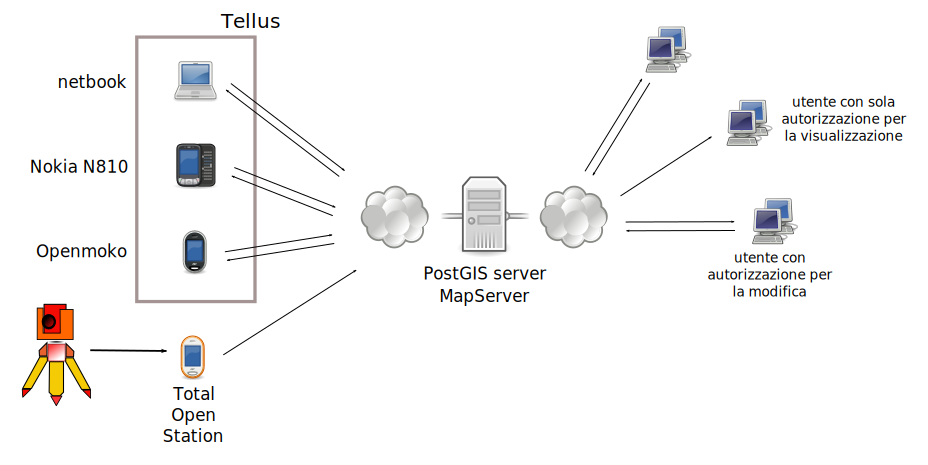
\includegraphics[scale=0.6]{img/tellus/schema_tellus}
			\caption{\label{fig:schema_tellus}{\small Raffigurazione schematica di un'infrastruttura di GIS mobile atta all'impiego in ambito archeologico.}}
		\end{figure}
	\end{center}

		\chapter{Listati di codice}

\section{raster\_tree.sh\label{sec:raster_tree.sh}}
\lstinputlisting[language=bash]{cap/code/raster_tree.sh}

		\chapter{Proiezioni\label{cha:Proiezioni}}


	\backmatter
	\include{cap/licence}
	%\chapter*{Sitografia e link}

Informazioni e link su sistemi GIS open source

\href{http://freegis.org}{http://freegis.org}\\
Modello del terreno (DTM) dell'intero pianeta

\href{http://www.ngdc.noaa.gov/mgg/topo/gltiles.html}{http://www.ngdc.noaa.gov/mgg/topo/gltiles.html}\\
GRASS GIS Homepage

\href{http://grass.itc.it/index.php}{http://grass.itc.it/index.php}\\
GRASS GIS Wiki, in inglese, pagina {}``Archeology''

\href{http://grass.osgeo.org/wiki/Archeology}{http://grass.osgeo.org/wiki/Archeology}\\
GRASS GIS Wiki in italiano, a cura di Gfoss.it

\href{http://wiki.gfoss.it}{http://wiki.gfoss.it}\\
GRASS per Microsoft Windows

\href{http://geni.ath.cx/grass.html}{http://geni.ath.cx/grass.html}\\
Tutorial su GRASS ed NVIZ

\href{http://www.ing.unitn.it/~grass/docs/tutorial/italiano}{http://www.ing.unitn.it/$\sim$grass/docs/tutorial/italiano}\\
Georeferenziazione di carte con GRASS GIS

\href{http://www.gis3w.it/download/manuali/georef_grass.pdf}{http://www.gis3w.it/download/manuali/georef\_{}grass.pdf}\\
Enciclopedia libera

\href{http://it.wikipedia.org}{http://it.wikipedia.org}\\
OpenStreetMap, la mappa mondiale libera in stile wiki

\href{http://www.openstreetmap.org}{http://www.openstreetmap.org}\\



\section*{Altre risorse}

Canale IRC internazionale di GRASS:

server \textsf{FreeNode}, canale \#grass\\
Mailing list internazionale di GRASS:

Iscrizione su \href{http://grass.itc.it/community/support.php\#int_list}{http://grass.itc.it/community/support.php\#{}int\_{}list},
indirizzo: \href{mailto:GRASSLIST@baylor.edu}{GRASSLIST@baylor.edu}.

\end{document}
